\RequirePackage{fix-cm} % fix some latex issues see: http://texdoc.net/texmf-dist/doc/latex/base/fixltx2e.pdf
\documentclass[twoside,openright,titlepage,numbers=noenddot,headinclude,%1headlines,% letterpaper a4paper
                footinclude=true,cleardoublepage=empty,abstractoff, % <--- obsolete, remove (todo)
                BCOR=5mm,paper=a4,fontsize=11pt,%11pt,a4paper,%
                ngerman,american,%
                ]{scrreprt}
% ****************************************************************************************************
% classicthesis-config.tex 
% formerly known as loadpackages.sty, classicthesis-ldpkg.sty, and classicthesis-preamble.sty 
% Use it at the beginning of your ClassicThesis.tex, or as a LaTeX Preamble 
% in your ClassicThesis.{tex,lyx} with % ****************************************************************************************************
% classicthesis-config.tex 
% formerly known as loadpackages.sty, classicthesis-ldpkg.sty, and classicthesis-preamble.sty 
% Use it at the beginning of your ClassicThesis.tex, or as a LaTeX Preamble 
% in your ClassicThesis.{tex,lyx} with % ****************************************************************************************************
% classicthesis-config.tex 
% formerly known as loadpackages.sty, classicthesis-ldpkg.sty, and classicthesis-preamble.sty 
% Use it at the beginning of your ClassicThesis.tex, or as a LaTeX Preamble 
% in your ClassicThesis.{tex,lyx} with \input{classicthesis-config}
% ****************************************************************************************************  
% If you like the classicthesis, then I would appreciate a postcard. 
% My address can be found in the file ClassicThesis.pdf. A collection 
% of the postcards I received so far is available online at 
% http://postcards.miede.de
% ****************************************************************************************************


% ****************************************************************************************************
% 0. Set the encoding of your files. UTF-8 is the only sensible encoding nowadays. If you can't read
% äöüßáéçèê∂åëæƒÏ€ then change the encoding setting in your editor, not the line below. If your editor
% does not support utf8 use another editor!
% ****************************************************************************************************
\PassOptionsToPackage{usenames,dvipsnames}{xcolor}%needed because several packages include xcolor
\PassOptionsToPackage{utf8}{inputenc}
\usepackage{inputenc}
        
% ****************************************************************************************************
% 1. Configure classicthesis for your needs here, e.g., remove "drafting" below 
% in order to deactivate the time-stamp on the pages
% ****************************************************************************************************
\PassOptionsToPackage{eulerchapternumbers,listings,%drafting,%
					 pdfspacing,%floatperchapter,%linedheaders,%
					 subfig,beramono,eulermath,parts}{classicthesis}                                        
% ********************************************************************
% Available options for classicthesis.sty 
% (see ClassicThesis.pdf for more information):
% drafting
% parts nochapters linedheaders
% eulerchapternumbers beramono eulermath pdfspacing minionprospacing
% tocaligned dottedtoc manychapters
% listings floatperchapter subfig
% ********************************************************************

\usepackage{url}
\usepackage{nameref}
\usepackage{datetime} %needed to add the date just below
\usepackage{pdflscape} %used to rotate pages with wide tables
\usepackage{rotating} %used to rotate wide figures
\usepackage{siunitx} %used for nice number formatting
\usepackage{pgf} % needed for arrays among other things
% ****************************************************************************************************
% 2. Personal data and user ad-hoc commands
% ****************************************************************************************************

\def\authors{
  {Luis Rodríguez Rubio/Student ID 1},
  {Sam Martin Vargas Giagnocavo/Student ID 2}}
\def\myTitle{Experimental CS Thesis Title\xspace}
\def\mySubtitle{A Guide for Content \& Style\xspace}
\def\myDegree{Project in Bioinformatics\xspace}
\def\myShortNames{Sam\xspace}
\def\myGroup{}
%\newcommand{\myStudentId}{20051234\xspace}
%\newcommand{\myNameToo}{Put Other Student Name Here\xspace}
%\newcommand{\myStudentIdToo}{20051235\xspace}
\def\myProf{Christian Storm Pederson\xspace}
\def\myOtherProf{Put name here\xspace}
\def\mySupervisor{Put name here\xspace}
\def\myFaculty{Faculty of Natural Sciences\xspace}
\def\myDepartment{Bioinformatics Research Centre\xspace}
\def\myUni{Aarhus University\xspace}
\def\myLocation{Aarhus\xspace}
\def\myTime{\monthname\ \the\year\xspace}
\def\myVersion{\xspace}


% ********************************************************************
% Setup, finetuning, and useful commands
% ********************************************************************
\newcounter{dummy} % necessary for correct hyperlinks (to index, bib, etc.)
\newlength{\abcd} % for ab..z string length calculation
\providecommand{\mLyX}{L\kern-.1667em\lower.25em\hbox{Y}\kern-.125emX\@}
\providecommand{\mBibTeX}{\textsc{Bib}\negthinspace\TeX\@}
% ****************************************************************************************************


% ****************************************************************************************************
% 3. Loading some handy packages
% ****************************************************************************************************
% ******************************************************************** 
% Packages with options that might require adjustments
% ******************************************************************** 
%\PassOptionsToPackage{ngerman,american}{babel}   % change this to your language(s)
% Spanish languages need extra options in order to work with this template
%\PassOptionsToPackage{spanish,es-lcroman}{babel}
\usepackage[american]{babel}                  
\usepackage{microtype}
\usepackage{csquotes}
\usepackage{ragged2e}
% \usepackage[usenames,dvipsnames]{xcolor}
\usepackage{xcolor}
\usepackage{pgf-umlsd}
\usepackage{pgfplots}
\usepackage{pgfplotstable}
% recommended:
\usepackage{booktabs}
\usepackage{array}
\usepackage{colortbl}
% \usepackage{color}
\definecolor{aublue}{HTML}{193b77} % the dark blue colour used by AU



%\usepackage[square,numbers,sort&compress]{natbib}
%\bibliographystyle{abbrvnat}

\PassOptionsToPackage{%
   %backend=biber, %instead of bibtex
	backend=bibtex8,bibencoding=ascii,%
	language=auto,%
	style=numeric-comp,%
   %style=authoryear-comp, % Author 1999, 2010
   %bibstyle=authoryear,dashed=false, % dashed: substitute rep. author with ---
   sorting=nyt, % name, year, title
   maxbibnames=10, % default: 3, et al.
   %backref=true,%
   natbib=true % natbib compatibility mode (\citep and \citet still work)
}{biblatex}
\usepackage{biblatex}

\PassOptionsToPackage{fleqn}{amsmath}       % math environments and more by the AMS 
\usepackage{amsmath}
%
% ******************************************************************** 
% General useful packages
% ******************************************************************** 
\PassOptionsToPackage{T1}{fontenc} % T2A for cyrillics
\usepackage{fontenc}     
\usepackage{textcomp} % fix warning with missing font shapes
\usepackage{scrhack} % fix warnings when using KOMA with listings package          
\usepackage{xspace} % to get the spacing after macros right  
\newcommand{\eg}{e.g.,\xspace}
\newcommand{\Eg}{E.g.,\xspace}
\newcommand{\etal}{et~al.\xspace}
\newcommand{\etc}{etc.\@\xspace}
\newcommand{\ie}{i.e.,\xspace}
\newcommand{\viz}{viz.\@\xspace}

\usepackage{mparhack} % get marginpar right
\usepackage{fixltx2e} % fixes some LaTeX stuff --> since 2015 in the LaTeX kernel (see below)
%\usepackage[latest]{latexrelease} % will be used once available in more distributions (ISSUE #107)
\PassOptionsToPackage{printonlyused,smaller}{acronym} 
    \usepackage{acronym} % nice macros for handling all acronyms in the thesis
    %\renewcommand{\bflabel}[1]{{#1}\hfill} % fix the list of acronyms --> no longer working
    %\renewcommand*{\acsfont}[1]{\textsc{#1}} 
    \renewcommand*{\aclabelfont}[1]{\acsfont{#1}}
% ****************************************************************************************************


% ****************************************************************************************************
% 4. Setup floats: tables, (sub)figures, and captions
% ****************************************************************************************************
\usepackage{tabularx} % better tables
    \setlength{\extrarowheight}{3pt} % increase table row height
\newcommand{\tableheadline}[1]{\multicolumn{1}{c}{\spacedlowsmallcaps{#1}}}
\newcommand{\myfloatalign}{\centering} % to be used with each float for alignment
\usepackage{caption}
% Thanks to cgnieder and Claus Lahiri
% http://tex.stackexchange.com/questions/69349/spacedlowsmallcaps-in-caption-label
% [REMOVED DUE TO OTHER PROBLEMS, SEE ISSUE #82]    
%\DeclareCaptionLabelFormat{smallcaps}{\bothIfFirst{#1}{~}\MakeTextLowercase{\textsc{#2}}}
%\captionsetup{font=small,labelformat=smallcaps} % format=hang,
\captionsetup{font=small} % format=hang,
\usepackage{subfig}  
% ****************************************************************************************************


% ****************************************************************************************************
% 5. Setup code listings
% ****************************************************************************************************
\usepackage{listings} 
%\lstset{emph={trueIndex,root},emphstyle=\color{BlueViolet}}%\underbar} % for special keywords
\lstset{language=[LaTeX]Tex,%C++,
    morekeywords={PassOptionsToPackage,selectlanguage},
    keywordstyle=\color{RoyalBlue},%\bfseries,
    basicstyle=\small\ttfamily,
    identifierstyle=\color{NavyBlue},
    commentstyle=\color{Green}\ttfamily,
    stringstyle=\rmfamily,
    numbers=left,
    numberstyle=\tiny\color{Gray},
    stepnumber=1,
    numbersep=8pt,
    showstringspaces=false,
    breaklines=true,
    %frameround=ftff,
    %frame=single,
    belowcaptionskip=.75\baselineskip
    %frame=L
} 
% ****************************************************************************************************             


% ****************************************************************************************************
% 6. PDFLaTeX, hyperreferences and citation backreferences
% ****************************************************************************************************
% ********************************************************************
% Using PDFLaTeX
% ********************************************************************
\PassOptionsToPackage{pdftex,hyperfootnotes=false,pdfpagelabels}{hyperref}
    \usepackage{hyperref}  % backref linktocpage pagebackref
\pdfcompresslevel=9
\pdfadjustspacing=1 
\PassOptionsToPackage{pdftex}{graphicx}
    \usepackage{graphicx} 
 

% ********************************************************************
% Hyperreferences
% ********************************************************************
\hypersetup{%
    %draft, % = no hyperlinking at all (useful in b/w printouts)
    colorlinks=true, linktocpage=true, pdfstartpage=3, pdfstartview=FitV,%
    % uncomment the following line if you want to have black links (e.g., for printing)
    %colorlinks=false, linktocpage=false, pdfstartpage=3, pdfstartview=FitV, pdfborder={0 0 0},%
    breaklinks=true, pdfpagemode=UseNone, pageanchor=true, pdfpagemode=UseOutlines,%
    plainpages=false, bookmarksnumbered, bookmarksopen=true, bookmarksopenlevel=1,%
    hypertexnames=true, pdfhighlight=/O,%nesting=true,%frenchlinks,%
    urlcolor=webbrown, linkcolor=RoyalBlue, citecolor=webgreen, %pagecolor=RoyalBlue,%
    %urlcolor=Black, linkcolor=Black, citecolor=Black, %pagecolor=Black,%
    pdftitle={\myTitle},%
    pdfauthor={\textcopyright\ \myShortNames, \myUni, \myFaculty},%
    pdfsubject={},%
    pdfkeywords={},%
    pdfcreator={pdfLaTeX},%
    pdfproducer={LaTeX with hyperref and classicthesis}%
}   

% ********************************************************************
% Setup autoreferences
% ********************************************************************
% There are some issues regarding autorefnames
% http://www.ureader.de/msg/136221647.aspx
% http://www.tex.ac.uk/cgi-bin/texfaq2html?label=latexwords
% you have to redefine the makros for the 
% language you use, e.g., american, ngerman
% (as chosen when loading babel/AtBeginDocument)
% ********************************************************************
\makeatletter
\@ifpackageloaded{babel}%
    {%
       \addto\extrasamerican{%
			\renewcommand*{\figureautorefname}{Figure}%
			\renewcommand*{\tableautorefname}{Table}%
			\renewcommand*{\partautorefname}{Part}%
			\renewcommand*{\chapterautorefname}{Chapter}%
			\renewcommand*{\sectionautorefname}{Section}%
			\renewcommand*{\subsectionautorefname}{Section}%
			\renewcommand*{\subsubsectionautorefname}{Section}%     
                }%
       \addto\extrasngerman{% 
			\renewcommand*{\paragraphautorefname}{Absatz}%
			\renewcommand*{\subparagraphautorefname}{Unterabsatz}%
			\renewcommand*{\footnoteautorefname}{Fu\"snote}%
			\renewcommand*{\FancyVerbLineautorefname}{Zeile}%
			\renewcommand*{\theoremautorefname}{Theorem}%
			\renewcommand*{\appendixautorefname}{Anhang}%
			\renewcommand*{\equationautorefname}{Gleichung}%        
			\renewcommand*{\itemautorefname}{Punkt}%
                }%  
            % Fix to getting autorefs for subfigures right (thanks to Belinda Vogt for changing the definition)
            \providecommand{\subfigureautorefname}{\figureautorefname}%             
    }{\relax}
\makeatother


% ****************************************************************************************************
% 7. Last calls before the bar closes
% ****************************************************************************************************
% ********************************************************************
% Development Stuff
% ********************************************************************
\listfiles
%\PassOptionsToPackage{l2tabu,orthodox,abort}{nag}
%   \usepackage{nag}
%\PassOptionsToPackage{warning, all}{onlyamsmath}
%   \usepackage{onlyamsmath}

% ********************************************************************
% Last, but not least...
% ********************************************************************
\usepackage{classicthesis} 
% ****************************************************************************************************


% ****************************************************************************************************
% 8. Further adjustments (experimental)
% ****************************************************************************************************
% ********************************************************************
% Changing the text area
% ********************************************************************
%\linespread{1.05} % a bit more for Palatino
%\areaset[current]{312pt}{761pt} % 686 (factor 2.2) + 33 head + 42 head \the\footskip
%\setlength{\marginparwidth}{7em}%
%\setlength{\marginparsep}{2em}%

% ********************************************************************
% Using different fonts
% ********************************************************************
%\usepackage[oldstylenums]{kpfonts} % oldstyle notextcomp
%\usepackage[osf]{libertine}
%\usepackage[light,condensed,math]{iwona}
%\renewcommand{\sfdefault}{iwona}
%\usepackage{lmodern} % <-- no osf support :-(
%\usepackage{cfr-lm} % 
%\usepackage[urw-garamond]{mathdesign} <-- no osf support :-(
%\usepackage[default,osfigures]{opensans} % scale=0.95 
%\usepackage[sfdefault]{FiraSans}
% ****************************************************************************************************



%%% Local Variables:
%%% mode: latex
%%% TeX-master: "./ClassicThesis"
%%% End:

% ****************************************************************************************************  
% If you like the classicthesis, then I would appreciate a postcard. 
% My address can be found in the file ClassicThesis.pdf. A collection 
% of the postcards I received so far is available online at 
% http://postcards.miede.de
% ****************************************************************************************************


% ****************************************************************************************************
% 0. Set the encoding of your files. UTF-8 is the only sensible encoding nowadays. If you can't read
% äöüßáéçèê∂åëæƒÏ€ then change the encoding setting in your editor, not the line below. If your editor
% does not support utf8 use another editor!
% ****************************************************************************************************
\PassOptionsToPackage{usenames,dvipsnames}{xcolor}%needed because several packages include xcolor
\PassOptionsToPackage{utf8}{inputenc}
\usepackage{inputenc}
        
% ****************************************************************************************************
% 1. Configure classicthesis for your needs here, e.g., remove "drafting" below 
% in order to deactivate the time-stamp on the pages
% ****************************************************************************************************
\PassOptionsToPackage{eulerchapternumbers,listings,%drafting,%
					 pdfspacing,%floatperchapter,%linedheaders,%
					 subfig,beramono,eulermath,parts}{classicthesis}                                        
% ********************************************************************
% Available options for classicthesis.sty 
% (see ClassicThesis.pdf for more information):
% drafting
% parts nochapters linedheaders
% eulerchapternumbers beramono eulermath pdfspacing minionprospacing
% tocaligned dottedtoc manychapters
% listings floatperchapter subfig
% ********************************************************************

\usepackage{url}
\usepackage{nameref}
\usepackage{datetime} %needed to add the date just below
\usepackage{pdflscape} %used to rotate pages with wide tables
\usepackage{rotating} %used to rotate wide figures
\usepackage{siunitx} %used for nice number formatting
\usepackage{pgf} % needed for arrays among other things
% ****************************************************************************************************
% 2. Personal data and user ad-hoc commands
% ****************************************************************************************************

\def\authors{
  {Luis Rodríguez Rubio/Student ID 1},
  {Sam Martin Vargas Giagnocavo/Student ID 2}}
\def\myTitle{Experimental CS Thesis Title\xspace}
\def\mySubtitle{A Guide for Content \& Style\xspace}
\def\myDegree{Project in Bioinformatics\xspace}
\def\myShortNames{Sam\xspace}
\def\myGroup{}
%\newcommand{\myStudentId}{20051234\xspace}
%\newcommand{\myNameToo}{Put Other Student Name Here\xspace}
%\newcommand{\myStudentIdToo}{20051235\xspace}
\def\myProf{Christian Storm Pederson\xspace}
\def\myOtherProf{Put name here\xspace}
\def\mySupervisor{Put name here\xspace}
\def\myFaculty{Faculty of Natural Sciences\xspace}
\def\myDepartment{Bioinformatics Research Centre\xspace}
\def\myUni{Aarhus University\xspace}
\def\myLocation{Aarhus\xspace}
\def\myTime{\monthname\ \the\year\xspace}
\def\myVersion{\xspace}


% ********************************************************************
% Setup, finetuning, and useful commands
% ********************************************************************
\newcounter{dummy} % necessary for correct hyperlinks (to index, bib, etc.)
\newlength{\abcd} % for ab..z string length calculation
\providecommand{\mLyX}{L\kern-.1667em\lower.25em\hbox{Y}\kern-.125emX\@}
\providecommand{\mBibTeX}{\textsc{Bib}\negthinspace\TeX\@}
% ****************************************************************************************************


% ****************************************************************************************************
% 3. Loading some handy packages
% ****************************************************************************************************
% ******************************************************************** 
% Packages with options that might require adjustments
% ******************************************************************** 
%\PassOptionsToPackage{ngerman,american}{babel}   % change this to your language(s)
% Spanish languages need extra options in order to work with this template
%\PassOptionsToPackage{spanish,es-lcroman}{babel}
\usepackage[american]{babel}                  
\usepackage{microtype}
\usepackage{csquotes}
\usepackage{ragged2e}
% \usepackage[usenames,dvipsnames]{xcolor}
\usepackage{xcolor}
\usepackage{pgf-umlsd}
\usepackage{pgfplots}
\usepackage{pgfplotstable}
% recommended:
\usepackage{booktabs}
\usepackage{array}
\usepackage{colortbl}
% \usepackage{color}
\definecolor{aublue}{HTML}{193b77} % the dark blue colour used by AU



%\usepackage[square,numbers,sort&compress]{natbib}
%\bibliographystyle{abbrvnat}

\PassOptionsToPackage{%
   %backend=biber, %instead of bibtex
	backend=bibtex8,bibencoding=ascii,%
	language=auto,%
	style=numeric-comp,%
   %style=authoryear-comp, % Author 1999, 2010
   %bibstyle=authoryear,dashed=false, % dashed: substitute rep. author with ---
   sorting=nyt, % name, year, title
   maxbibnames=10, % default: 3, et al.
   %backref=true,%
   natbib=true % natbib compatibility mode (\citep and \citet still work)
}{biblatex}
\usepackage{biblatex}

\PassOptionsToPackage{fleqn}{amsmath}       % math environments and more by the AMS 
\usepackage{amsmath}
%
% ******************************************************************** 
% General useful packages
% ******************************************************************** 
\PassOptionsToPackage{T1}{fontenc} % T2A for cyrillics
\usepackage{fontenc}     
\usepackage{textcomp} % fix warning with missing font shapes
\usepackage{scrhack} % fix warnings when using KOMA with listings package          
\usepackage{xspace} % to get the spacing after macros right  
\newcommand{\eg}{e.g.,\xspace}
\newcommand{\Eg}{E.g.,\xspace}
\newcommand{\etal}{et~al.\xspace}
\newcommand{\etc}{etc.\@\xspace}
\newcommand{\ie}{i.e.,\xspace}
\newcommand{\viz}{viz.\@\xspace}

\usepackage{mparhack} % get marginpar right
\usepackage{fixltx2e} % fixes some LaTeX stuff --> since 2015 in the LaTeX kernel (see below)
%\usepackage[latest]{latexrelease} % will be used once available in more distributions (ISSUE #107)
\PassOptionsToPackage{printonlyused,smaller}{acronym} 
    \usepackage{acronym} % nice macros for handling all acronyms in the thesis
    %\renewcommand{\bflabel}[1]{{#1}\hfill} % fix the list of acronyms --> no longer working
    %\renewcommand*{\acsfont}[1]{\textsc{#1}} 
    \renewcommand*{\aclabelfont}[1]{\acsfont{#1}}
% ****************************************************************************************************


% ****************************************************************************************************
% 4. Setup floats: tables, (sub)figures, and captions
% ****************************************************************************************************
\usepackage{tabularx} % better tables
    \setlength{\extrarowheight}{3pt} % increase table row height
\newcommand{\tableheadline}[1]{\multicolumn{1}{c}{\spacedlowsmallcaps{#1}}}
\newcommand{\myfloatalign}{\centering} % to be used with each float for alignment
\usepackage{caption}
% Thanks to cgnieder and Claus Lahiri
% http://tex.stackexchange.com/questions/69349/spacedlowsmallcaps-in-caption-label
% [REMOVED DUE TO OTHER PROBLEMS, SEE ISSUE #82]    
%\DeclareCaptionLabelFormat{smallcaps}{\bothIfFirst{#1}{~}\MakeTextLowercase{\textsc{#2}}}
%\captionsetup{font=small,labelformat=smallcaps} % format=hang,
\captionsetup{font=small} % format=hang,
\usepackage{subfig}  
% ****************************************************************************************************


% ****************************************************************************************************
% 5. Setup code listings
% ****************************************************************************************************
\usepackage{listings} 
%\lstset{emph={trueIndex,root},emphstyle=\color{BlueViolet}}%\underbar} % for special keywords
\lstset{language=[LaTeX]Tex,%C++,
    morekeywords={PassOptionsToPackage,selectlanguage},
    keywordstyle=\color{RoyalBlue},%\bfseries,
    basicstyle=\small\ttfamily,
    identifierstyle=\color{NavyBlue},
    commentstyle=\color{Green}\ttfamily,
    stringstyle=\rmfamily,
    numbers=left,
    numberstyle=\tiny\color{Gray},
    stepnumber=1,
    numbersep=8pt,
    showstringspaces=false,
    breaklines=true,
    %frameround=ftff,
    %frame=single,
    belowcaptionskip=.75\baselineskip
    %frame=L
} 
% ****************************************************************************************************             


% ****************************************************************************************************
% 6. PDFLaTeX, hyperreferences and citation backreferences
% ****************************************************************************************************
% ********************************************************************
% Using PDFLaTeX
% ********************************************************************
\PassOptionsToPackage{pdftex,hyperfootnotes=false,pdfpagelabels}{hyperref}
    \usepackage{hyperref}  % backref linktocpage pagebackref
\pdfcompresslevel=9
\pdfadjustspacing=1 
\PassOptionsToPackage{pdftex}{graphicx}
    \usepackage{graphicx} 
 

% ********************************************************************
% Hyperreferences
% ********************************************************************
\hypersetup{%
    %draft, % = no hyperlinking at all (useful in b/w printouts)
    colorlinks=true, linktocpage=true, pdfstartpage=3, pdfstartview=FitV,%
    % uncomment the following line if you want to have black links (e.g., for printing)
    %colorlinks=false, linktocpage=false, pdfstartpage=3, pdfstartview=FitV, pdfborder={0 0 0},%
    breaklinks=true, pdfpagemode=UseNone, pageanchor=true, pdfpagemode=UseOutlines,%
    plainpages=false, bookmarksnumbered, bookmarksopen=true, bookmarksopenlevel=1,%
    hypertexnames=true, pdfhighlight=/O,%nesting=true,%frenchlinks,%
    urlcolor=webbrown, linkcolor=RoyalBlue, citecolor=webgreen, %pagecolor=RoyalBlue,%
    %urlcolor=Black, linkcolor=Black, citecolor=Black, %pagecolor=Black,%
    pdftitle={\myTitle},%
    pdfauthor={\textcopyright\ \myShortNames, \myUni, \myFaculty},%
    pdfsubject={},%
    pdfkeywords={},%
    pdfcreator={pdfLaTeX},%
    pdfproducer={LaTeX with hyperref and classicthesis}%
}   

% ********************************************************************
% Setup autoreferences
% ********************************************************************
% There are some issues regarding autorefnames
% http://www.ureader.de/msg/136221647.aspx
% http://www.tex.ac.uk/cgi-bin/texfaq2html?label=latexwords
% you have to redefine the makros for the 
% language you use, e.g., american, ngerman
% (as chosen when loading babel/AtBeginDocument)
% ********************************************************************
\makeatletter
\@ifpackageloaded{babel}%
    {%
       \addto\extrasamerican{%
			\renewcommand*{\figureautorefname}{Figure}%
			\renewcommand*{\tableautorefname}{Table}%
			\renewcommand*{\partautorefname}{Part}%
			\renewcommand*{\chapterautorefname}{Chapter}%
			\renewcommand*{\sectionautorefname}{Section}%
			\renewcommand*{\subsectionautorefname}{Section}%
			\renewcommand*{\subsubsectionautorefname}{Section}%     
                }%
       \addto\extrasngerman{% 
			\renewcommand*{\paragraphautorefname}{Absatz}%
			\renewcommand*{\subparagraphautorefname}{Unterabsatz}%
			\renewcommand*{\footnoteautorefname}{Fu\"snote}%
			\renewcommand*{\FancyVerbLineautorefname}{Zeile}%
			\renewcommand*{\theoremautorefname}{Theorem}%
			\renewcommand*{\appendixautorefname}{Anhang}%
			\renewcommand*{\equationautorefname}{Gleichung}%        
			\renewcommand*{\itemautorefname}{Punkt}%
                }%  
            % Fix to getting autorefs for subfigures right (thanks to Belinda Vogt for changing the definition)
            \providecommand{\subfigureautorefname}{\figureautorefname}%             
    }{\relax}
\makeatother


% ****************************************************************************************************
% 7. Last calls before the bar closes
% ****************************************************************************************************
% ********************************************************************
% Development Stuff
% ********************************************************************
\listfiles
%\PassOptionsToPackage{l2tabu,orthodox,abort}{nag}
%   \usepackage{nag}
%\PassOptionsToPackage{warning, all}{onlyamsmath}
%   \usepackage{onlyamsmath}

% ********************************************************************
% Last, but not least...
% ********************************************************************
\usepackage{classicthesis} 
% ****************************************************************************************************


% ****************************************************************************************************
% 8. Further adjustments (experimental)
% ****************************************************************************************************
% ********************************************************************
% Changing the text area
% ********************************************************************
%\linespread{1.05} % a bit more for Palatino
%\areaset[current]{312pt}{761pt} % 686 (factor 2.2) + 33 head + 42 head \the\footskip
%\setlength{\marginparwidth}{7em}%
%\setlength{\marginparsep}{2em}%

% ********************************************************************
% Using different fonts
% ********************************************************************
%\usepackage[oldstylenums]{kpfonts} % oldstyle notextcomp
%\usepackage[osf]{libertine}
%\usepackage[light,condensed,math]{iwona}
%\renewcommand{\sfdefault}{iwona}
%\usepackage{lmodern} % <-- no osf support :-(
%\usepackage{cfr-lm} % 
%\usepackage[urw-garamond]{mathdesign} <-- no osf support :-(
%\usepackage[default,osfigures]{opensans} % scale=0.95 
%\usepackage[sfdefault]{FiraSans}
% ****************************************************************************************************



%%% Local Variables:
%%% mode: latex
%%% TeX-master: "./ClassicThesis"
%%% End:

% ****************************************************************************************************  
% If you like the classicthesis, then I would appreciate a postcard. 
% My address can be found in the file ClassicThesis.pdf. A collection 
% of the postcards I received so far is available online at 
% http://postcards.miede.de
% ****************************************************************************************************


% ****************************************************************************************************
% 0. Set the encoding of your files. UTF-8 is the only sensible encoding nowadays. If you can't read
% äöüßáéçèê∂åëæƒÏ€ then change the encoding setting in your editor, not the line below. If your editor
% does not support utf8 use another editor!
% ****************************************************************************************************
\PassOptionsToPackage{usenames,dvipsnames}{xcolor}%needed because several packages include xcolor
\PassOptionsToPackage{utf8}{inputenc}
\usepackage{inputenc}
        
% ****************************************************************************************************
% 1. Configure classicthesis for your needs here, e.g., remove "drafting" below 
% in order to deactivate the time-stamp on the pages
% ****************************************************************************************************
\PassOptionsToPackage{eulerchapternumbers,listings,%drafting,%
					 pdfspacing,%floatperchapter,%linedheaders,%
					 subfig,beramono,eulermath,parts}{classicthesis}                                        
% ********************************************************************
% Available options for classicthesis.sty 
% (see ClassicThesis.pdf for more information):
% drafting
% parts nochapters linedheaders
% eulerchapternumbers beramono eulermath pdfspacing minionprospacing
% tocaligned dottedtoc manychapters
% listings floatperchapter subfig
% ********************************************************************

\usepackage{url}
\usepackage{nameref}
\usepackage{datetime} %needed to add the date just below
\usepackage{pdflscape} %used to rotate pages with wide tables
\usepackage{rotating} %used to rotate wide figures
\usepackage{siunitx} %used for nice number formatting
\usepackage{pgf} % needed for arrays among other things
% ****************************************************************************************************
% 2. Personal data and user ad-hoc commands
% ****************************************************************************************************

\def\authors{
  {Luis Rodríguez Rubio/Student ID 1},
  {Sam Martin Vargas Giagnocavo/Student ID 2}}
\def\myTitle{Experimental CS Thesis Title\xspace}
\def\mySubtitle{A Guide for Content \& Style\xspace}
\def\myDegree{Project in Bioinformatics\xspace}
\def\myShortNames{Sam\xspace}
\def\myGroup{}
%\newcommand{\myStudentId}{20051234\xspace}
%\newcommand{\myNameToo}{Put Other Student Name Here\xspace}
%\newcommand{\myStudentIdToo}{20051235\xspace}
\def\myProf{Christian Storm Pederson\xspace}
\def\myOtherProf{Put name here\xspace}
\def\mySupervisor{Put name here\xspace}
\def\myFaculty{Faculty of Natural Sciences\xspace}
\def\myDepartment{Bioinformatics Research Centre\xspace}
\def\myUni{Aarhus University\xspace}
\def\myLocation{Aarhus\xspace}
\def\myTime{\monthname\ \the\year\xspace}
\def\myVersion{\xspace}


% ********************************************************************
% Setup, finetuning, and useful commands
% ********************************************************************
\newcounter{dummy} % necessary for correct hyperlinks (to index, bib, etc.)
\newlength{\abcd} % for ab..z string length calculation
\providecommand{\mLyX}{L\kern-.1667em\lower.25em\hbox{Y}\kern-.125emX\@}
\providecommand{\mBibTeX}{\textsc{Bib}\negthinspace\TeX\@}
% ****************************************************************************************************


% ****************************************************************************************************
% 3. Loading some handy packages
% ****************************************************************************************************
% ******************************************************************** 
% Packages with options that might require adjustments
% ******************************************************************** 
%\PassOptionsToPackage{ngerman,american}{babel}   % change this to your language(s)
% Spanish languages need extra options in order to work with this template
%\PassOptionsToPackage{spanish,es-lcroman}{babel}
\usepackage[american]{babel}                  
\usepackage{microtype}
\usepackage{csquotes}
\usepackage{ragged2e}
% \usepackage[usenames,dvipsnames]{xcolor}
\usepackage{xcolor}
\usepackage{pgf-umlsd}
\usepackage{pgfplots}
\usepackage{pgfplotstable}
% recommended:
\usepackage{booktabs}
\usepackage{array}
\usepackage{colortbl}
% \usepackage{color}
\definecolor{aublue}{HTML}{193b77} % the dark blue colour used by AU



%\usepackage[square,numbers,sort&compress]{natbib}
%\bibliographystyle{abbrvnat}

\PassOptionsToPackage{%
   %backend=biber, %instead of bibtex
	backend=bibtex8,bibencoding=ascii,%
	language=auto,%
	style=numeric-comp,%
   %style=authoryear-comp, % Author 1999, 2010
   %bibstyle=authoryear,dashed=false, % dashed: substitute rep. author with ---
   sorting=nyt, % name, year, title
   maxbibnames=10, % default: 3, et al.
   %backref=true,%
   natbib=true % natbib compatibility mode (\citep and \citet still work)
}{biblatex}
\usepackage{biblatex}

\PassOptionsToPackage{fleqn}{amsmath}       % math environments and more by the AMS 
\usepackage{amsmath}
%
% ******************************************************************** 
% General useful packages
% ******************************************************************** 
\PassOptionsToPackage{T1}{fontenc} % T2A for cyrillics
\usepackage{fontenc}     
\usepackage{textcomp} % fix warning with missing font shapes
\usepackage{scrhack} % fix warnings when using KOMA with listings package          
\usepackage{xspace} % to get the spacing after macros right  
\newcommand{\eg}{e.g.,\xspace}
\newcommand{\Eg}{E.g.,\xspace}
\newcommand{\etal}{et~al.\xspace}
\newcommand{\etc}{etc.\@\xspace}
\newcommand{\ie}{i.e.,\xspace}
\newcommand{\viz}{viz.\@\xspace}

\usepackage{mparhack} % get marginpar right
\usepackage{fixltx2e} % fixes some LaTeX stuff --> since 2015 in the LaTeX kernel (see below)
%\usepackage[latest]{latexrelease} % will be used once available in more distributions (ISSUE #107)
\PassOptionsToPackage{printonlyused,smaller}{acronym} 
    \usepackage{acronym} % nice macros for handling all acronyms in the thesis
    %\renewcommand{\bflabel}[1]{{#1}\hfill} % fix the list of acronyms --> no longer working
    %\renewcommand*{\acsfont}[1]{\textsc{#1}} 
    \renewcommand*{\aclabelfont}[1]{\acsfont{#1}}
% ****************************************************************************************************


% ****************************************************************************************************
% 4. Setup floats: tables, (sub)figures, and captions
% ****************************************************************************************************
\usepackage{tabularx} % better tables
    \setlength{\extrarowheight}{3pt} % increase table row height
\newcommand{\tableheadline}[1]{\multicolumn{1}{c}{\spacedlowsmallcaps{#1}}}
\newcommand{\myfloatalign}{\centering} % to be used with each float for alignment
\usepackage{caption}
% Thanks to cgnieder and Claus Lahiri
% http://tex.stackexchange.com/questions/69349/spacedlowsmallcaps-in-caption-label
% [REMOVED DUE TO OTHER PROBLEMS, SEE ISSUE #82]    
%\DeclareCaptionLabelFormat{smallcaps}{\bothIfFirst{#1}{~}\MakeTextLowercase{\textsc{#2}}}
%\captionsetup{font=small,labelformat=smallcaps} % format=hang,
\captionsetup{font=small} % format=hang,
\usepackage{subfig}  
% ****************************************************************************************************


% ****************************************************************************************************
% 5. Setup code listings
% ****************************************************************************************************
\usepackage{listings} 
%\lstset{emph={trueIndex,root},emphstyle=\color{BlueViolet}}%\underbar} % for special keywords
\lstset{language=[LaTeX]Tex,%C++,
    morekeywords={PassOptionsToPackage,selectlanguage},
    keywordstyle=\color{RoyalBlue},%\bfseries,
    basicstyle=\small\ttfamily,
    identifierstyle=\color{NavyBlue},
    commentstyle=\color{Green}\ttfamily,
    stringstyle=\rmfamily,
    numbers=left,
    numberstyle=\tiny\color{Gray},
    stepnumber=1,
    numbersep=8pt,
    showstringspaces=false,
    breaklines=true,
    %frameround=ftff,
    %frame=single,
    belowcaptionskip=.75\baselineskip
    %frame=L
} 
% ****************************************************************************************************             


% ****************************************************************************************************
% 6. PDFLaTeX, hyperreferences and citation backreferences
% ****************************************************************************************************
% ********************************************************************
% Using PDFLaTeX
% ********************************************************************
\PassOptionsToPackage{pdftex,hyperfootnotes=false,pdfpagelabels}{hyperref}
    \usepackage{hyperref}  % backref linktocpage pagebackref
\pdfcompresslevel=9
\pdfadjustspacing=1 
\PassOptionsToPackage{pdftex}{graphicx}
    \usepackage{graphicx} 
 

% ********************************************************************
% Hyperreferences
% ********************************************************************
\hypersetup{%
    %draft, % = no hyperlinking at all (useful in b/w printouts)
    colorlinks=true, linktocpage=true, pdfstartpage=3, pdfstartview=FitV,%
    % uncomment the following line if you want to have black links (e.g., for printing)
    %colorlinks=false, linktocpage=false, pdfstartpage=3, pdfstartview=FitV, pdfborder={0 0 0},%
    breaklinks=true, pdfpagemode=UseNone, pageanchor=true, pdfpagemode=UseOutlines,%
    plainpages=false, bookmarksnumbered, bookmarksopen=true, bookmarksopenlevel=1,%
    hypertexnames=true, pdfhighlight=/O,%nesting=true,%frenchlinks,%
    urlcolor=webbrown, linkcolor=RoyalBlue, citecolor=webgreen, %pagecolor=RoyalBlue,%
    %urlcolor=Black, linkcolor=Black, citecolor=Black, %pagecolor=Black,%
    pdftitle={\myTitle},%
    pdfauthor={\textcopyright\ \myShortNames, \myUni, \myFaculty},%
    pdfsubject={},%
    pdfkeywords={},%
    pdfcreator={pdfLaTeX},%
    pdfproducer={LaTeX with hyperref and classicthesis}%
}   

% ********************************************************************
% Setup autoreferences
% ********************************************************************
% There are some issues regarding autorefnames
% http://www.ureader.de/msg/136221647.aspx
% http://www.tex.ac.uk/cgi-bin/texfaq2html?label=latexwords
% you have to redefine the makros for the 
% language you use, e.g., american, ngerman
% (as chosen when loading babel/AtBeginDocument)
% ********************************************************************
\makeatletter
\@ifpackageloaded{babel}%
    {%
       \addto\extrasamerican{%
			\renewcommand*{\figureautorefname}{Figure}%
			\renewcommand*{\tableautorefname}{Table}%
			\renewcommand*{\partautorefname}{Part}%
			\renewcommand*{\chapterautorefname}{Chapter}%
			\renewcommand*{\sectionautorefname}{Section}%
			\renewcommand*{\subsectionautorefname}{Section}%
			\renewcommand*{\subsubsectionautorefname}{Section}%     
                }%
       \addto\extrasngerman{% 
			\renewcommand*{\paragraphautorefname}{Absatz}%
			\renewcommand*{\subparagraphautorefname}{Unterabsatz}%
			\renewcommand*{\footnoteautorefname}{Fu\"snote}%
			\renewcommand*{\FancyVerbLineautorefname}{Zeile}%
			\renewcommand*{\theoremautorefname}{Theorem}%
			\renewcommand*{\appendixautorefname}{Anhang}%
			\renewcommand*{\equationautorefname}{Gleichung}%        
			\renewcommand*{\itemautorefname}{Punkt}%
                }%  
            % Fix to getting autorefs for subfigures right (thanks to Belinda Vogt for changing the definition)
            \providecommand{\subfigureautorefname}{\figureautorefname}%             
    }{\relax}
\makeatother


% ****************************************************************************************************
% 7. Last calls before the bar closes
% ****************************************************************************************************
% ********************************************************************
% Development Stuff
% ********************************************************************
\listfiles
%\PassOptionsToPackage{l2tabu,orthodox,abort}{nag}
%   \usepackage{nag}
%\PassOptionsToPackage{warning, all}{onlyamsmath}
%   \usepackage{onlyamsmath}

% ********************************************************************
% Last, but not least...
% ********************************************************************
\usepackage{classicthesis} 
% ****************************************************************************************************


% ****************************************************************************************************
% 8. Further adjustments (experimental)
% ****************************************************************************************************
% ********************************************************************
% Changing the text area
% ********************************************************************
%\linespread{1.05} % a bit more for Palatino
%\areaset[current]{312pt}{761pt} % 686 (factor 2.2) + 33 head + 42 head \the\footskip
%\setlength{\marginparwidth}{7em}%
%\setlength{\marginparsep}{2em}%

% ********************************************************************
% Using different fonts
% ********************************************************************
%\usepackage[oldstylenums]{kpfonts} % oldstyle notextcomp
%\usepackage[osf]{libertine}
%\usepackage[light,condensed,math]{iwona}
%\renewcommand{\sfdefault}{iwona}
%\usepackage{lmodern} % <-- no osf support :-(
%\usepackage{cfr-lm} % 
%\usepackage[urw-garamond]{mathdesign} <-- no osf support :-(
%\usepackage[default,osfigures]{opensans} % scale=0.95 
%\usepackage[sfdefault]{FiraSans}
% ****************************************************************************************************



%%% Local Variables:
%%% mode: latex
%%% TeX-master: "./ClassicThesis"
%%% End:


% Color packages
\usepackage{color,soul}

% Caption for subfigures
\usepackage{subcaption}

% FLoatBarrier
\usepackage{placeins}

% Equation conditions
\newenvironment{conditions}
  {\par\vspace{\abovedisplayskip}\noindent
   \begin{tabular}{>{$}l<{$} @{} >{${}}c<{{}$} @{} l}}
  {\end{tabular}\par\vspace{\belowdisplayskip}}

\newenvironment{conditions*}
  {\par\vspace{\abovedisplayskip}\noindent
   \tabularx{\columnwidth}{>{$}l<{$} @{}>{${}}c<{{}$}@{} >{\raggedright\arraybackslash}X}}
  {\endtabularx\par\vspace{\belowdisplayskip}}


% *********************************************************
% Change these values to match your group and project title
% *********************************************************
\def\myDegree{Project in Bioinformatics - 10 ECTS}
\def\myTitle{Minimum Spanning Trees as an alternative to Gusfield’s Guide Tree}
\def\mySubtitle{} % Maybe we should write something else here
\def\authors{
  {Luis Rodríguez Rubio/AU703347},
  {Sam Martin Vargas Giagnocavo/AU703393}}
\def\myShortNames{
    {Luis},
    {Sam}}
\def\myGroup{}

%********************************************************************
% Bibliographies
%*******************************************************
\addbibresource{Bibliography.bib}
\usepackage{amsmath}
\usepackage{algorithm} 
\usepackage{algpseudocode}
%********************************************************************
% Hyphenation
%*******************************************************
\hyphenation{Micro-soft Web-RTC Chun-ky-Spread Ka-dem-lia Pas-try mac-OS block-chain time-stamp Et-he-re-um}

% ********************************************************************
% GO!GO!GO! MOVE IT!
%*******************************************************
\begin{document}
\frenchspacing
\raggedbottom
\selectlanguage{american} % american ngerman
%\renewcommand*{\bibname}{new name}
%\setbibpreamble{}
\pagenumbering{roman}
\pagestyle{plain}
%********************************************************************
% Frontmatter
%*******************************************************
%*******************************************************
% Little Dirty Titlepage
%*******************************************************
\thispagestyle{empty}
%\pdfbookmark[1]{Titel}{title}
%*******************************************************
\vspace*{\fill}\noindent{\color{aublue}\rule{\linewidth}{1mm}\\[4ex]\color{black}
  \begin{RaggedRight}
\Large \spacedallcaps \myTitle\\ \vspace*{1.5em}
\large \spacedallcaps \mySubtitle\\ \vspace*{3em}
\end{RaggedRight}
\foreach \name\id in \authors
{
  {\noindent\Large \spacedlowsmallcaps \name, \id }\\[1ex]
}
\\[-1ex]
{\noindent\large \spacedlowsmallcaps \myGroup}\\[1.5ex]
\noindent\color{aublue}\rule{\linewidth}{1mm}\\[4ex]\color{black}
\noindent{\large \spacedlowsmallcaps \myDegree\\[1ex] 
\monthname\ \the\year  \\[1ex] Advisor: \myProf \\[23ex]}\\[\fill]}

\includegraphics[width=\linewidth]{gfx/logo}\clearpage


%*******************************************************
% Titlepage
%*******************************************************
\begin{titlepage}
	% if you want the titlepage to be centered, uncomment and fine-tune the line below (KOMA classes environment)
	\begin{addmargin}[-1cm]{-3cm}
    \begin{center}
        \large  

        \hfill

        \vfill

        \begingroup
            \color{Maroon}\spacedallcaps{\myTitle} \\ \bigskip
        \endgroup
        \emph{\mySubtitle} \\ \medskip

        \spacedlowsmallcaps{\myShortNames}\\

        \vfill

        
\includegraphics[width=6cm]{gfx/au-logo} \\ \medskip

        \myDegree \\ \medskip
        \myDepartment \\                            
        \myFaculty \\
        \myUni \\ \bigskip

        \myTime

        \vfill                      

    \end{center}  
  \end{addmargin}       
\end{titlepage}   
\thispagestyle{empty}

\hfill

\vfill

\noindent\myShortNames: \textit{\myTitle,} \myDegree
\ \textcopyright\ \myTime

%\bigskip
%
%\noindent\spacedlowsmallcaps{Supervisors}: \\
%\myProf \\
%\myOtherProf \\ 
%\mySupervisor
%
%\medskip
%
%\noindent\spacedlowsmallcaps{Location}: \\
%\myLocation
%
%\medskip
%
%\noindent\spacedlowsmallcaps{Time Frame}: \\
%\myTime

\pagestyle{scrheadings}
\cleardoublepage\include{FrontBackmatter/Contents}
%********************************************************************
% Mainmatter
%*******************************************************
\cleardoublepage\pagenumbering{arabic}
\cleardoublepage

\chapter{Introduction}
\label{cha:introduction}

% Spacing between paragraphs
\setlength{\parskip}{5pt plus2pt}

Multiple sequence alignment remains one of the most cost intensive tasks in bio-informatics. Finding the optimal score for multiple sequences can prove challenging even in scenarios involving a reduced number of short sequences.

In order to find the optimal solution, as in any naïve implementation, the algorithm has to check for all of the possible combinations at a certain position in the alignment, thus considerably increasing the complexity of the problem for each evaluated sequence in the final alignment.

In addition, depending on how the algorithm defines the cost (or score) to be, the complexity of the algorithm will build up to an even greater extent. Different strategies exist, such as the \textit{sum-of-pairs} score, which computes the score of the entire alignment by computing the score for each of the columns (see \textit{Equation \ref{eq:sum-of-pairs}}). Unfortunately, it can prove problematic in certain situations where one sequence - or a small number sequences - skews the score in an otherwise perfect alignment. Other scoring functions like the \textit{consensus score} or \textit{tree score} exist but only as an alternative to the widely used \textit{sum-of-pairs} score used in most of the multiple-sequence-alignment workloads \cite{fu-berlin}.

\begin{equation}\label{eq:sum-of-pairs}
    SP\;Score = \sum_{c = 0}^{n} \sum_{i = 0}^{k} \sum_{\substack{j = 0 \\ j > i}}^{k} g_{c}(i,j)
\end{equation}
where:
\begin{conditions}
 n     & =       &  Length of the alignment (number of columns) \\
 k & = & Number of sequences in the alignment \\ 
 g_{c} & = & Cost function at specific column with sequence i and j
\end{conditions}

As for what concerns the project, \textit{sum-of-pairs} will be the chosen cost function since the goal is to improve and build upon the \textit{Gusfields} algorithm, which uses the aforementioned function. As a result, all references to scoring functions or optimal scores throughout the document will be referring or resulting from the \textit{sum-of-pairs} score.

Having specified the scoring methodology that will be used, a comprehensive definition of the naïve algorithm can be made.

Say the optimal alignment for $k$ sequences of $n$ length each needs to be found, since the \textit{sum-of-pairs} score is a column-based scoring function, all of the different possibilities need to be evaluated (which in this case is $2$, one for a new gap and another for the current character). 

The \textit{sum-of-pairs} score is additive, so the algorithm needs to keep track of whatever was scored previously - the dynamic programming approach (see \textit{Figure \ref{fig:dp-msa}} for a sketch of the process). This results on an algorithm that needs to fill out $n^{k}$ cells each representing a column, trying $2^{k}-1$ combinations\footnote{A column can't be completely made up of gaps, therefore one combination has to be subtracted from the total.} for each column and evaluating each combination with $k^{2}-1$ comparisons\footnote{This assumes $cost(A,B) = cost(B,A)$.}. The total running time amounts to a massive $O(n^{k} * (2^{k}-1) * (k^{2}-1))$ with a space consumption of $O(n^{k})$ in order to store the values.

\begin{figure}
    \centering
    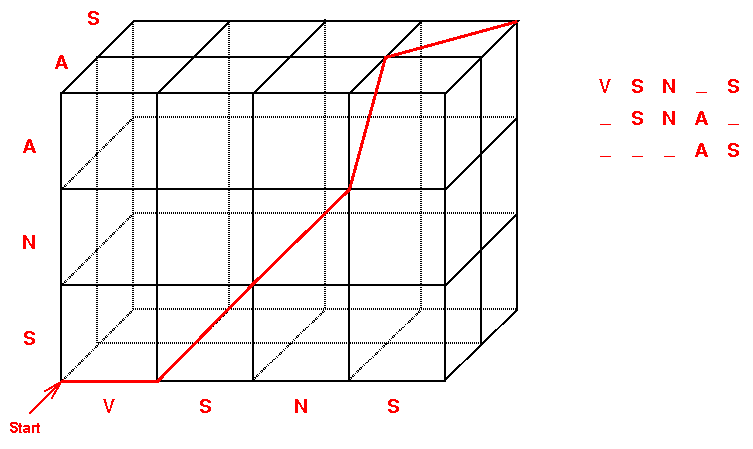
\includegraphics[width=7cm]{report/dp-msa.png}
    \caption{Optimal path of three sequences in a hyperlattice representation. Image extracted from \url{bioinfo3d.cs.tau.ac.il}.}
    \label{fig:dp-msa}
\end{figure}
 
Consequently, methods that use heuristics and offer near-optimal results receive the utmost attention in multiple sequencing workloads. Multiple sequence alignment is an NP-complete problem after all, to which no polynomial time solution exists \cite{cornell-msa}.

Amongst powerful solutions such as ClustalW - a progressive algorithm - we find the Gusfields 2-approximation algorithm: A simple algorithm which guarantees an alignment whose score is, at most, two times that of the optimal one \cite{fu-berlin} \cite{approx2}. 

The algorithm achieves this by choosing an order in which paired alignments of sequences are merged together to form the complete alignment. The order depends on finding a ``center sequence", the sequence the hast the least aggregate distance amongst all of the sequences we wish to align.

The $2 * OPTIMAL$ bound for the approximation algorithm can be demonstrated as follows. 

First we need to find an upper bound of the score for the computed alignment. In order to get the score we will use \textit{sum-of-pairs}, as we mentioned earlier. Then we will combine this upper bound (see \textit{Equation} \ref{eq:upper}) with the lower bound of the score for the optimal alignment (see \textit{Equation} \ref{eq:lower}). The factor resulting of dividing them will be our approximation.

\begin{equation}\label{eq:upper}
    \begin{split}
        SP(M) & = & \frac{1}{2}\sum_{i=1}^{k}\sum_{j=1,i\neq j}^{k}Score(M(S_i,S_j)) \\
 & = & \frac{1}{2}\sum_{i=1}^{k}\sum_{j=1,i\neq j}^{k}d(i,j) \\
 & \le  & \frac{1}{2}\sum_{i=1}^{k}\sum_{j=1,i\neq j}^{k}(d(i,1)+d(1,j)) \\
 & = & \frac{1}{2}\sum_{i=1}^{k}\sum_{j=1,i\neq j}^{k}(d(1,i)+d(1,j)) \\
 & = & \frac{1}{2}\sum_{l=2}^{k}2(k-1)d(1,l) \\
 & = & (k-1)\sum_{l=2}^{k}Score(M(S_1,S_l)) \\
 & = & (k-1)\sum_{l=2}^{k}D(S_1,S_l)
    \end{split}
\end{equation}

\begin{equation}\label{eq:lower}
    \begin{split}
        SP(M^*) & = & \frac{1}{2}\sum_{i=1}^{k}\sum_{j=1,i\neq j}^{k}Score(M^*(S_i,S_j)) \\
 & = & \frac{1}{2}\sum_{i=1}^{k}\sum_{j=1,i\neq j}^{k}d^*(i,j) \\
 & \ge  & \frac{1}{2}\sum_{i=1}^{k}\sum_{j=1,i\neq j}^{k}D(S_i,S_j) \\
 & = & \frac{1}{2}\sum_{i=1}^{k}\sum_{j=1,i\neq j}^{k}D(S_1,S_j) \\
 & = & \frac{1}{2}k\sum_{j=1}^{k}D(S_1,S_j) \\
 & = & \frac{1}{2}k\sum_{l=2}^{k}D(S_1,S_l)
    \end{split}
\end{equation}

where:

\begin{conditions}
SP(M) & = & Sum of Pairs score for MSA in matrix M. \\
 M(S_i,S_j)     & = &  Induced alignment of sequences i and j present in a MSA matrix M. \\
 Score() & = & Score of a pairwise alignment. \\ 
 d(i,j) & = & Score(M(S_i,S_j) rewritten. \\
 D(S_i,S_j) & = & Optimal alignment between sequences i and j.
\end{conditions}

And by diving them between each other we get the inequality which amounts to $2$ as seen in \textit{Equation \ref{eq:final}} \cite{fu-berlin}.
\begin{equation}\label{eq:final}
    \frac{SP(M)}{SP(M^*)}\le \frac{(k-1)\sum_{l=2}^{k}D(S_1,S_l)}{\frac{1}{2}k\sum_{l=2}^{k}D(S_1,S_l)}=\frac{2(k-1)}{k} < 2
\end{equation}
 
In this project, we will explore improvements to Gusfield's merging order by using a minimum spanning tree algorithm. From the bio-informatics standpoint, the goal is to see if the most optimal graph of sequences - which is generated by the minimum spanning tree algorithm - is suitable and offers an improvement over the ``stock" merging order. And from the Computer Science standpoint, the goal will be to develop a solution that works both locally and in a website.

\chapter{Architecture \& Implementation}
\label{cha:arch--impl}

\section{The core implementation}

As mentioned before, our implementation tries to explore the result of using Minimal Spanning Trees as "guide trees" when calculating an approximation for a Multiple Sequence Alignment. More precisely we will test if Kruskal's algorithm \cite{Kruskal1956} can be used in different ways to improve the results from Gusfield's approach.

\subsection{Gusfield's algorithm \& Minimal Spanning Trees}

Both Gusfield's approach and our Minimal Spanning Trees implementation start from a common initial procedure which consist of calculating all of the pairwise alignments between every sequence in our set.

This can be understood as calculating every edge of an adjacency matrix of a fully connected graph where every node is a sequence we want to align as we can observe in \textit{Figure \ref{fig:fullyconnected}}.

\begin{figure}[h]
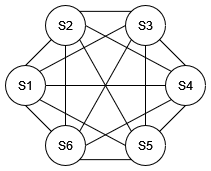
\includegraphics[width=4cm]{report/fullyconnected.png}
\centering
\caption{Fully connected graph were each node represent a unique sequence}
\label{fig:fullyconnected}
\end{figure}

This is the most computationally intensive section of the execution with a time complexity of \(O(k^2 \cdot n^2)\) being n the number of sequences we want to ailing and k their length.

After this part what both Gusfield and our Minimal Spaning Trees implementation do is find a tree within this graph to guide the Multiple Sequence Alignment. And the shape and methodology of creating this tree is the difference that we are going to explore.

In Gusfield's algorithm this guide tree is obtained first by finding the ``center string" of our adjacency matrix as mentioned in the 2-factor proof from the introduction. \textit{Equation \ref{eq:centerstring}} shows the process.

\begin{equation}\label{eq:centerstring}
\begin{aligned}
\text{Find }S_1 \text{ such that}\color{black} \sum_{S\in F-S_{1}}^{}Score(S_1,S) \color{Black} \text{ is minimized}\\
\text{Call the remaining strings } S_2, S_3, ..., S_k
\end{aligned}
\end{equation}

Once the center string has been found, we will connect every other sequence with this center string as we can observe in \textit{Figure \ref{fig:center_string}}.

\begin{figure}[h]
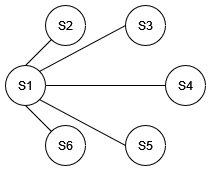
\includegraphics[width=4cm]{report/gusfields.png}
\centering
\caption{Tree obtained from joining every sequence to the Center String S1}
\label{fig:center_string}
\end{figure}

On the other hand, in our Minimal Spanning Trees approach we will build the tree following Kruskal's algorithm. The use of a MST as a guide tree should provide more information about the relationships between all the sequences in the alignment, hopefully allowing for a more accurate alignment. 

In comparison, a star-shaped tree, where the center string is the root and all other sequences are connected directly to the root, only considers the relationship between the center string and the other sequences and does not take into account the relationship between the other sequences. 

A MST is a tree that connects all the sequences in the alignment and has the minimum possible total edge weight. In this case our MST will be constructed using a pairwise distance matrix of the sequences, where the distance between two sequences is a measure of their similarity.

It's important to note that the use of a MST as a guide tree is not commonly used for MSA, as it doesn't have a theoretical guarantee for the alignment quality. Other alternatives such as progressive methods are more widely used.

A summary of Kruskal's algorithm to build a MST can be seen in \textit{pseudocode \ref{alg:kruskal}} \cite{cormen2022introduction}. One possible tree shape that we can obtain from Kruskal can be the one observed in \textit{Figure \ref{fig:mst_graph}}. Any resulting tree from the algorithm will not contain cycles.

\begin{algorithm}
	\caption{Kruskal's algorithm} 
    \label{alg:kruskal}
	\begin{algorithmic}[1]
        \State Order every edge on the fully connected graph by their weights.
        \State Edges are represented by the nodes they are connected to (u,v).
		\For {$(u, v) in ordered_edges$}
            \If {$(u,v) does not make a cycle when adding it to the tree$}
		          \State Add (u,v) to T.
		      \EndIf
		\EndFor
	\end{algorithmic} 
\end{algorithm}

\begin{figure}[h]
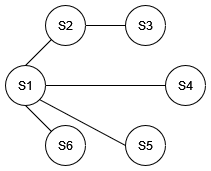
\includegraphics[width=4cm]{report/mst2.png}
\centering
\caption{Possible tree shape that can be obtained from Kruskal's algorithm}
\label{fig:mst_graph}
\end{figure}

From this point on, both algorithms follow their respective "guide tree" and add sequences one by one to the final alignment. In this case, the merging order in Kruskal would be determined by the the same merging order followed in \textit{pseudocode \ref{alg:kruskal}}.

This can be very easy to implement on the Gusfield's approach as every node is connected to the same one \cite{Gusfield_1997}. This detail makes that can add each sequence one by one in any order starting with the "center string". We can do this because the tree shape is going to follow this same characteristics every time, but we can not say the same about the Minimal Spanning Trees alternative.

With Minimal Spanning trees we wont always have the same tree shape. To deal with this problem of trying to find which node should we add at each step we modified Gusfield's implementation.

The matrix representing the multiple sequence alignment will be extended by merging matrix instead of only a single sequence to it.

Even though it is not part of our focus to optimize the execution, we implemented the Disjoint Set Union algorithm \cite{disjointsetunion} to build Kruskal's MST. This apart from being one of the fastest implementations is also very helpful with our goal of mixing sets of sequences together. Its main concept can be seen in \textit{pseudocode \ref{alg:kruskal-sets}}. 

\begin{algorithm}
	\caption{Kruskal's Disjoint Set Union} 
    \label{alg:kruskal-sets}
	\begin{algorithmic}[1]
        \State Initially make |V| single node sets
        \State Edges are represented by the nodes they are connected to (u,v).
		\For {$(u, v) in ordered_edges$}
            \State $S_u =$ set containing u
            \State $S_v =$ set containing v
            \If {$S_u$ is not the same as $S_v$}
		          \State add (u,v) to T
		      \EndIf
		\EndFor
	\end{algorithmic} 
\end{algorithm}

Here, u \& v are representing sequences, each one of them can be already in a bigger set which will be merged together.

Although computational complexity is not the primary focus of this implementation, it is worth noting that it does not significantly impact the running time. The Kruskal alternative may take slightly longer than Gusfield's method ($O(e \log V)$, $V$ being the number of vertices), but this difference is negligible. This is because the initial step of calculating the pairwise distance matrix is the most computationally intensive part of the process. Therefore, the time complexity remains the same for both Gusfield and our Kruskal alternatives, which is  \(O(k^2 \cdot n^2)\) where n is the number of sequences to be aligned and k is their length.

One key thing to note is the non-deterministic nature of our implementation in scenarios where sequences are reordered within the FASTA file. Currently, the adjacency matrix used for our Kruskal implementation computes all alignments as found in the FASTA file. This means that if a FASTA file contains sequences $S1$, $S2$ and $S3$ we will compare the sequences in the following order: $S1$ with $S2$, $S1$ with $S3$ and $S2$ with $S3$. However, if a variation of the FASTA file rearranges the sequences to $S3$, $S2$ and $S1$, the comparison will be the following: $S3$ with $S2$, $S3$ with $S1$ and $S2$ with $S1$. While distance is symmetrical, two sequences might have multiple alignments that share the same score. In our implementation there might be instances where depending on the arrangement of sequences in the FASTA files, different alignments will be used to merge the different clusters, resulting in a different final cluster and, consequently, score.

\subsection{Rust}

We decided to implement this algorithm using the Rust programming language. We did this because even though performance was not the primary focus we are interested in fast calculations and processing of the data to make the tool as usable as possible.

We also chose Rust instead other fast-performing languages because the reliability and memory safety as well as provide a WebAssembly package which we used to create our visualization web application. 

This has implied that along the duration of this project we learnt a new programming language with which we did not had any prior experience, and also learn how Web Assembly worked and how to include it in a web application.

During the development, our focus was on reusing as much code as possible for our two implementations, one as a CLI using Rust exclusively, and the other one calling Rust functions directly from JavaScript via WebAssembly.

We also focused on robustness and reliability working with error handling and edge cases along the way. We used GitHub's CD/CI capabilities to keep these principles in mind for every change committed to the repository (more insight into the configuration can be checked in \textit{section \ref{sec:github-ci}}). This required the project to be able to build and pass every unit test with each addition we made. Apart for unit testing we also added a benchmark framework to monitor and evaluate our running sequence. More information regarding the unit test and benchmarking features can be found on \textit{Chapter \ref{cha:evaluation}}.

\section{WebAssembly, our vessel to the Web}
As previously mentioned, we needed a programming language that would be flexible enough to allow for both a CLI and Web execution of the algorithm. Some options that were initially discussed included building an API and rewriting key sections of the CLI code in JavaScript. These were quickly discarded as WebAssembly would allow us to reuse a great part of the codebase.

WebAssembly acts as an intermediary between a number of supported programming languages (e.g. Python, C++, Rust, Go, etc.) and JavaScript by converting the original code into byte-code that can be run by most browsers used at the time of writing \cite{mdn-wasm}.

Converting the original code into the byte-code that needs to be called from JavaScript requires tools that are language-dependant. In the case of Rust, \href{https://github.com/rustwasm/wasm-pack}{\textit{wasm-pack}} is the tool to use.

Not all of the code is compiled into WebAssembly. The user has to be specify which functions have to be compiled by listing them in the \textit{lib.rs}\footnote{In our project we have renamed the file to \textit{wasm.rs} in order to reflect the main use of the file.} file and using a macro. An example can be seen in the following code listing:

\begin{lstlisting}[language=Rust,numbers=none]
#[wasm_bindgen]
pub fn wasm_serialize_fasta_string(fasta_string: String) -> JsValue {
    let sequences = parse_fasta_string(fasta_string);
    serde_wasm_bindgen::to_value(&sequences).unwrap()
}
\end{lstlisting}

In it's current state, WebAssembly in Rust does not offer a ``smooth" transition in most cases. Notice the use of the \lstinline[columns=fixed]{serde_wasm_bindgen} function.

One of the \href{https://github.com/rustwasm/wasm-bindgen/issues/111}{limitations that is still present at the time of writing the report} is the lack of any native option to return vectors storing custom \textit{structs} to JavaScript. Some workarounds, such as using a \textit{\&[u8]} type intermediary exist but are only valid for ``simpler" \textit{structures} that can be easily converted and parsed from an array of bytes. In our case, we make use of multiple nested structures so an alternative was needed.

As listed in the code above, \href{https://serde.rs/}{Serde} was the solution we decided to use. In this case, the workaround implemented from the library is using a JSON string as an intermediary. The problem in this case would be the need for the bare JavaScript code to parse the incoming arguments, adding an additional overhead to the web client. However, after brief tests we considered this a minor issue. If results from the WASM functions were too big to be parsed, other aspects of the website would also be harmed, regardless of the methodology for passing data between the WebAssembly and JavaScript code.

One of the other interesting alternatives that were explored included sharing a memory buffer between the Rust code - which ends up being converted to WebAssembly - and JavaScript code at all times. In the end, this option was discarded due to its complexity.

For the final version of the website all of the alignments were done in WebAssembly and parsed and displayed in JavaScript.

\section{Visualizing alignments}
With the ever-expanding state of the web we thought it would be interesting to take advantage of the flexibility and accessibility of the available programming tools and frameworks to display the process and steps of the alignment, something that is not easily done with popular languages in the desktop space such as C++, C\verb|#| and others.

Since we would be taking on a space - canvas visualization on the web - that we had no prior experience with, this part of development ended up being  prone to changes.

Initial designs and sketches for the website included the visualization of the guide tree with a live step by step display of the cluster alignments. After an initial review of the available JavaScript visualization libraries we decided to prioritize the step by step visualization of the alignments over displaying the graph. Unless we opted for a bare bones implementation there would not be a general framework or library that would easily allow us to implement both features, thus including both would require two different JavaScript libraries which would increase the complexity and maintainability of our solution. The chosen library for the implementation would end up being \href{https://createjs.com}{CreateJS}, a suite of inter-compatible JavaScript libraries.

Due to the design choices that were made at the initial stages of the project - e.g. working with the merge-order vectors - development of the user interface did not require having the command-line client finished. Early prototypes of the visualization can be seen in \textit{Figure \ref{fig:proto}}. Here we can see the three main stages the visualization goes through in order to complete a character-based alignment visualization. From left to right, the visualization displays two clusters that are joining together and a reference alignment used to guide the merging process (left-most image), an animation that starts moving parts of one cluster to another (center image) and finally the end result of the operation for that specific position. Note that \textit{Figure \ref{fig:proto}} shows an early prototype so the reference alignment used to guide the merging process is completely random and serves as a placeholder.

\begin{figure}%
    \centering
    \subfigure{
        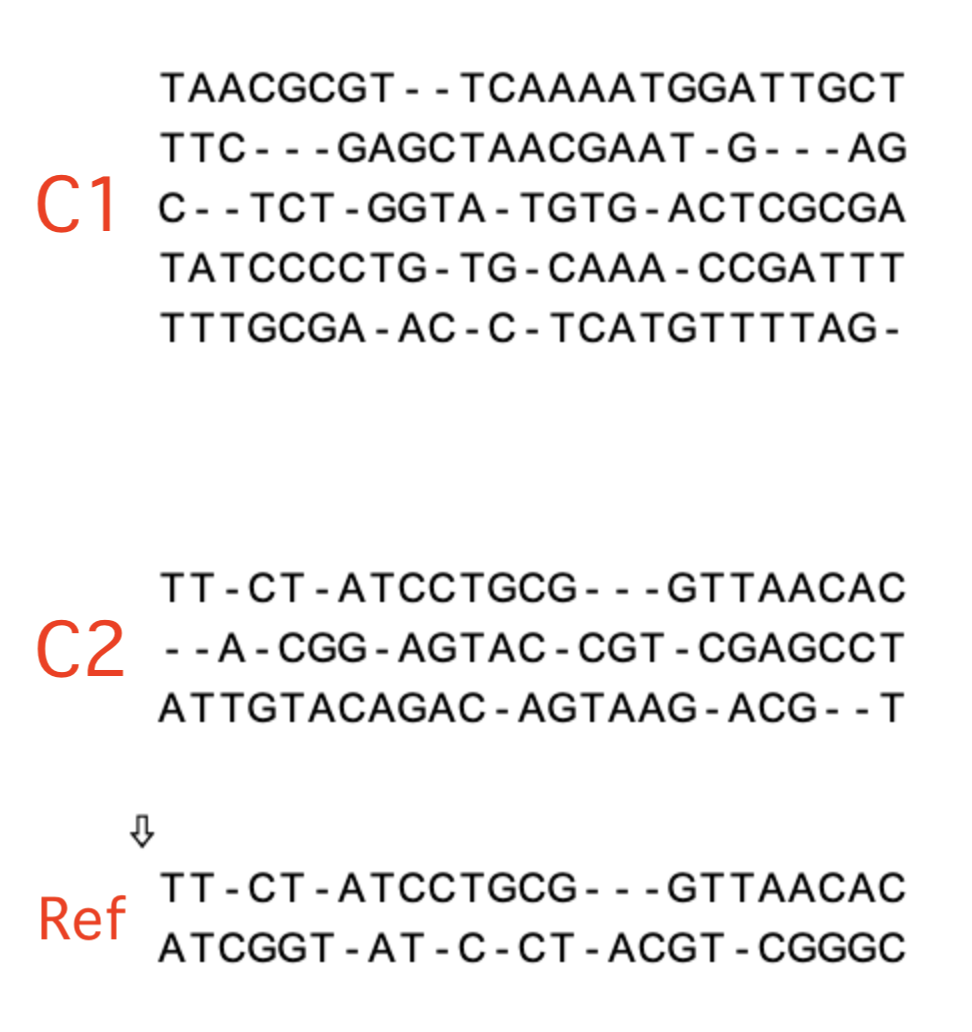
\includegraphics[width=3cm]{report/anim-align-1.png}
    }%
    \qquad
    \subfigure{
        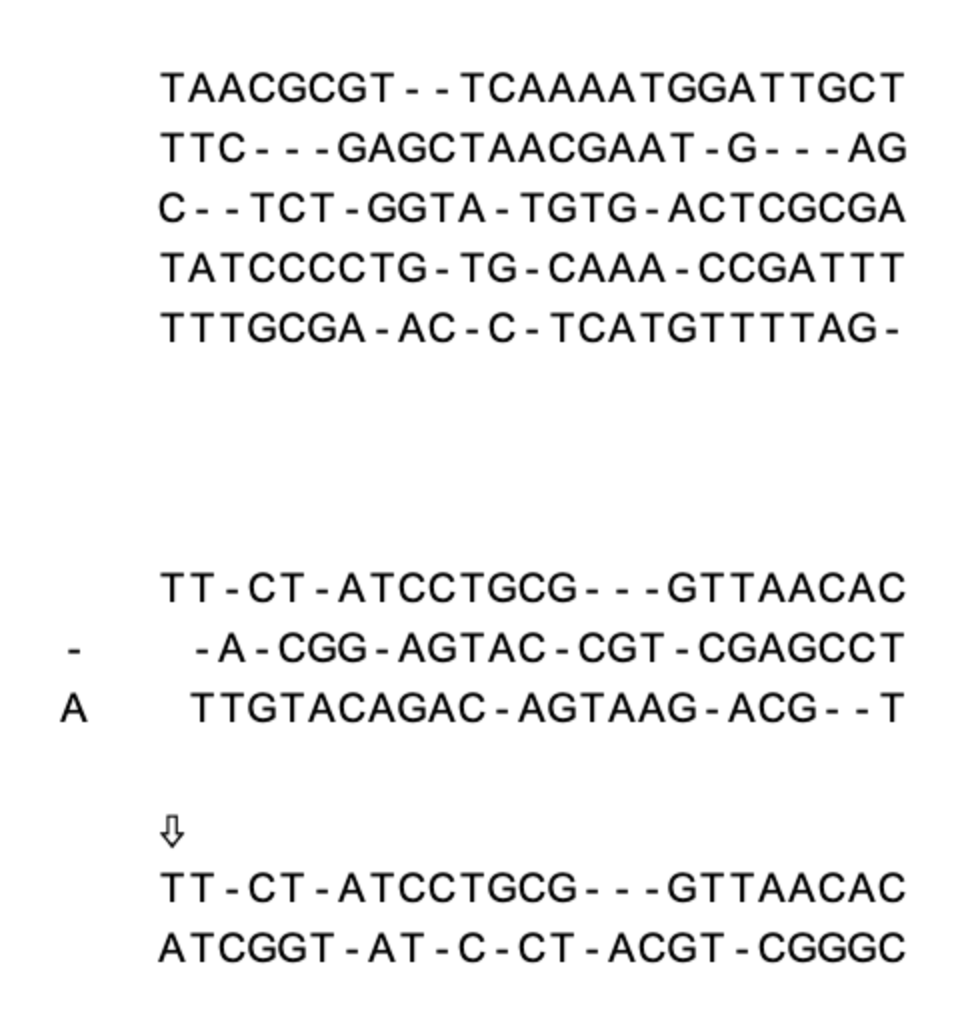
\includegraphics[width=3cm]{report/anim-align-2.png}
    }%
    \qquad
    \subfigure{
        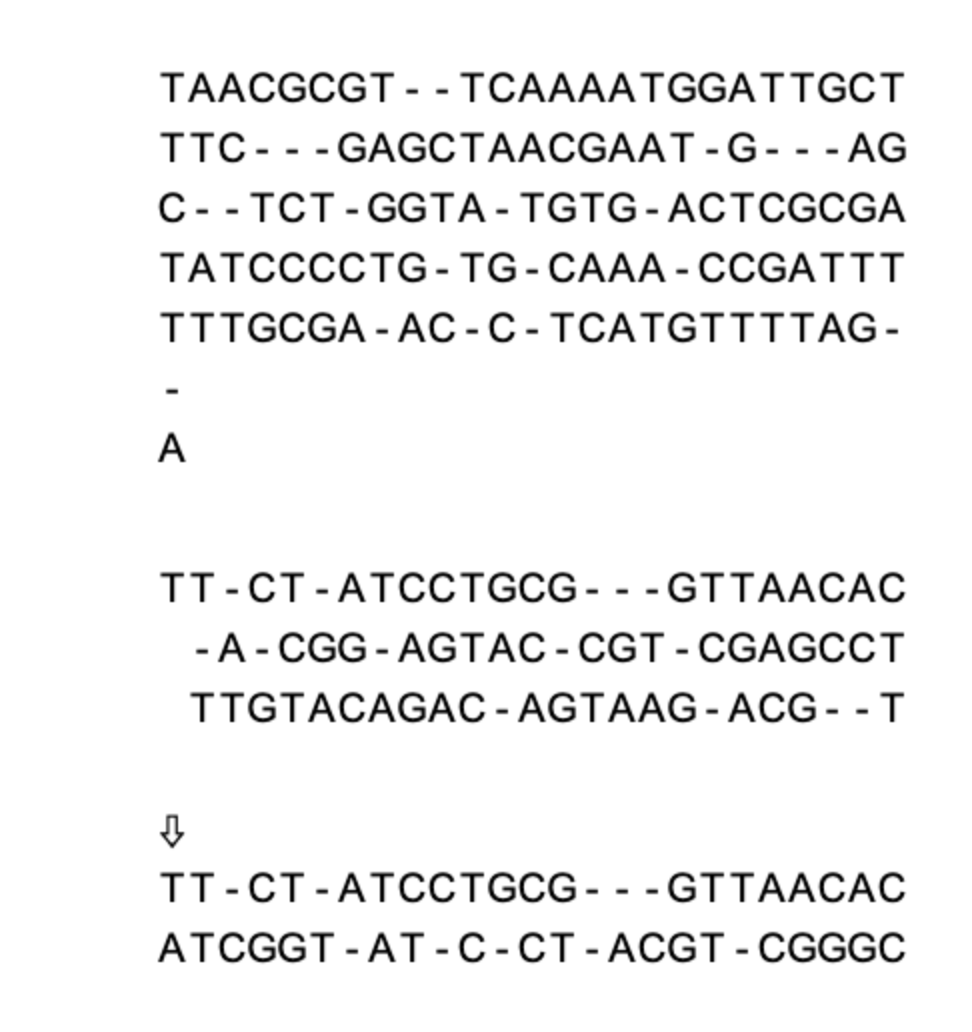
\includegraphics[width=3cm]{report/anim-align-3.png}
    }%
    \caption{Character-based steps animated in our first prototypes.}
    \label{fig:proto}
\end{figure}

As development of the Rust back-end continued, problems concerning the performance of the visualization were a concern. The initial approach that was taken, as suggested in \textit{Figure \ref{fig:proto}} was to have each character as a unit. The issue with this approach lies on the capabilities of the library to manage thousands of different ``sprites"\footnote{Term used to describe images that represent an asset.} at the same time, which in this case was not possible. Some optimizations, such as the removal of off-screen visualizations were attempted but even then, performance was sub-optimal.

Consequently, a simpler approach was taken which involved simply displaying and animating the three clusters from each step. At the beginning of each step the two clusters that are yet to be merged swipe from the right and after that the result swipes from the bottom. This process repeats itself until the visualization reaches the end and displays the resulting cluster with the sum-of-pairs score. \textit{Figure 6} shows the three main events in order.

\begin{figure}[h]%
    \centering
    \label{fig:anim-align-final}
    \subfigure{
        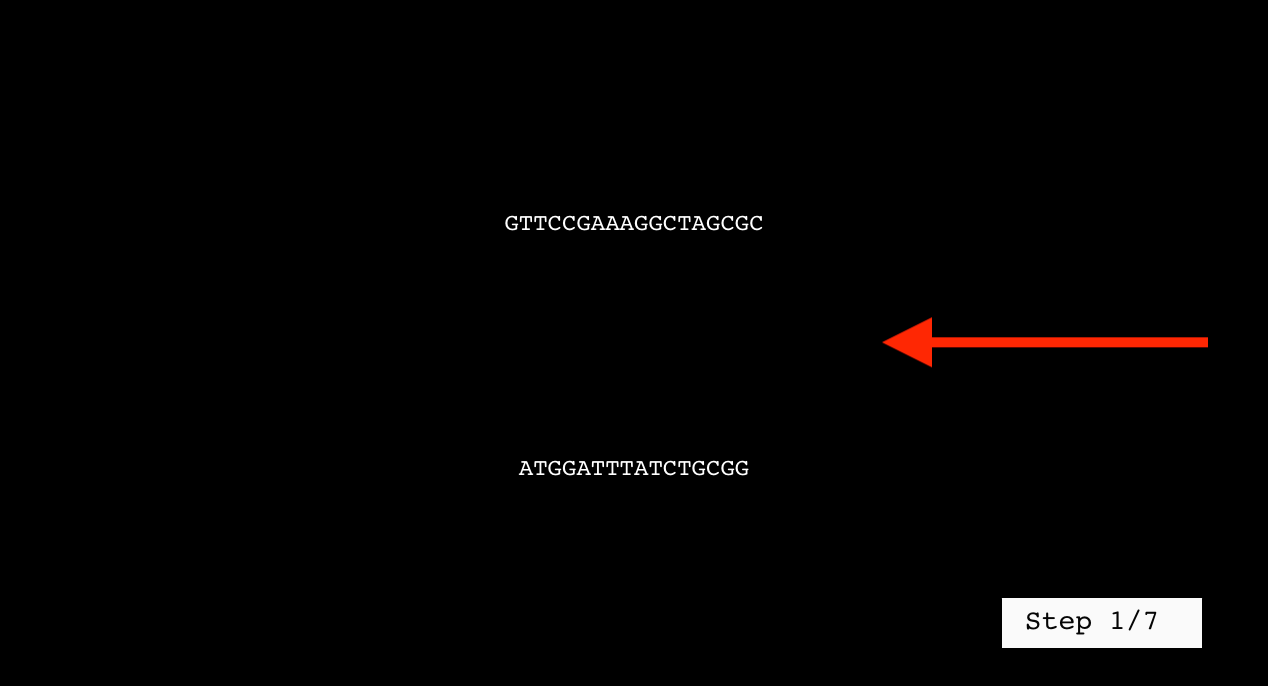
\includegraphics[width=6cm]{report/phase-1.png}
    }%
    
    \\
    
    \subfigure{
        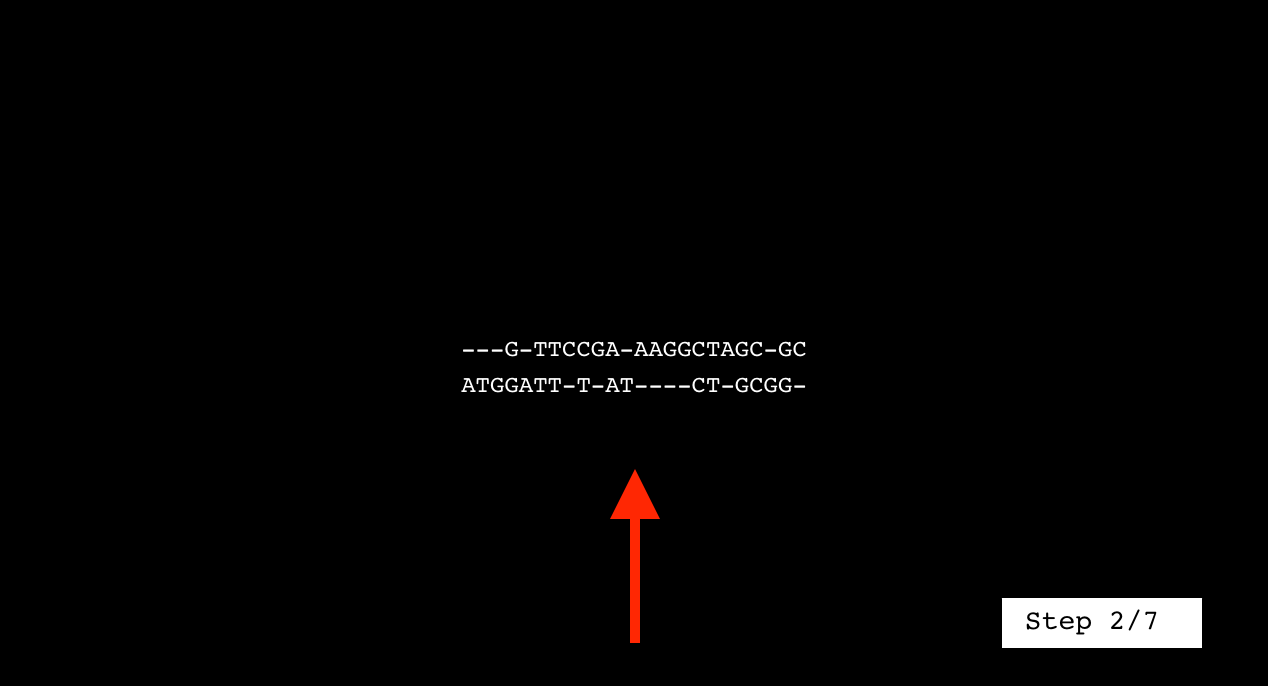
\includegraphics[width=6cm]{report/phase-2.png}
    }%
    
    \\
    
    \subfigure{
        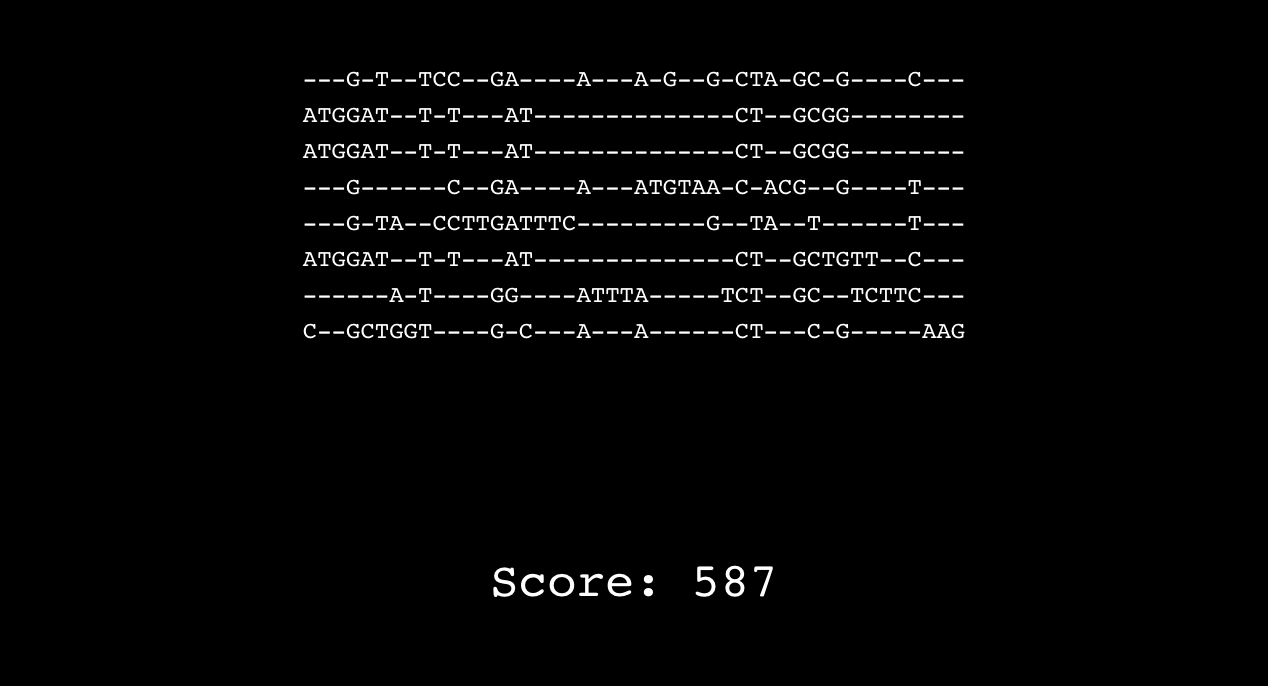
\includegraphics[width=6cm]{report/phase-end.png}
    }%
    \caption{Final visualization. As opposed to the initial prototypes, which manipulated individual characters, this only animates and moves clusters.}
    
\end{figure}

The website allows the user to configure all of the alignment parameters available in the command line program. Users can both, paste and select files containing sequences and cost matrices as seen in \textit{Figure \ref{fig:webapp}}. Once all of the data has been loaded and parameters have been set, users can click on the "PLAY" button to start the visualization. A slower alternative to the continuous visualization can be triggered by using the "STEP" button, which requires an interaction from the user per step. "TOGGLE" and "RESET" will toggle the on-going animation and remove all images from the canvas respectively.

\begin{figure}[h]
    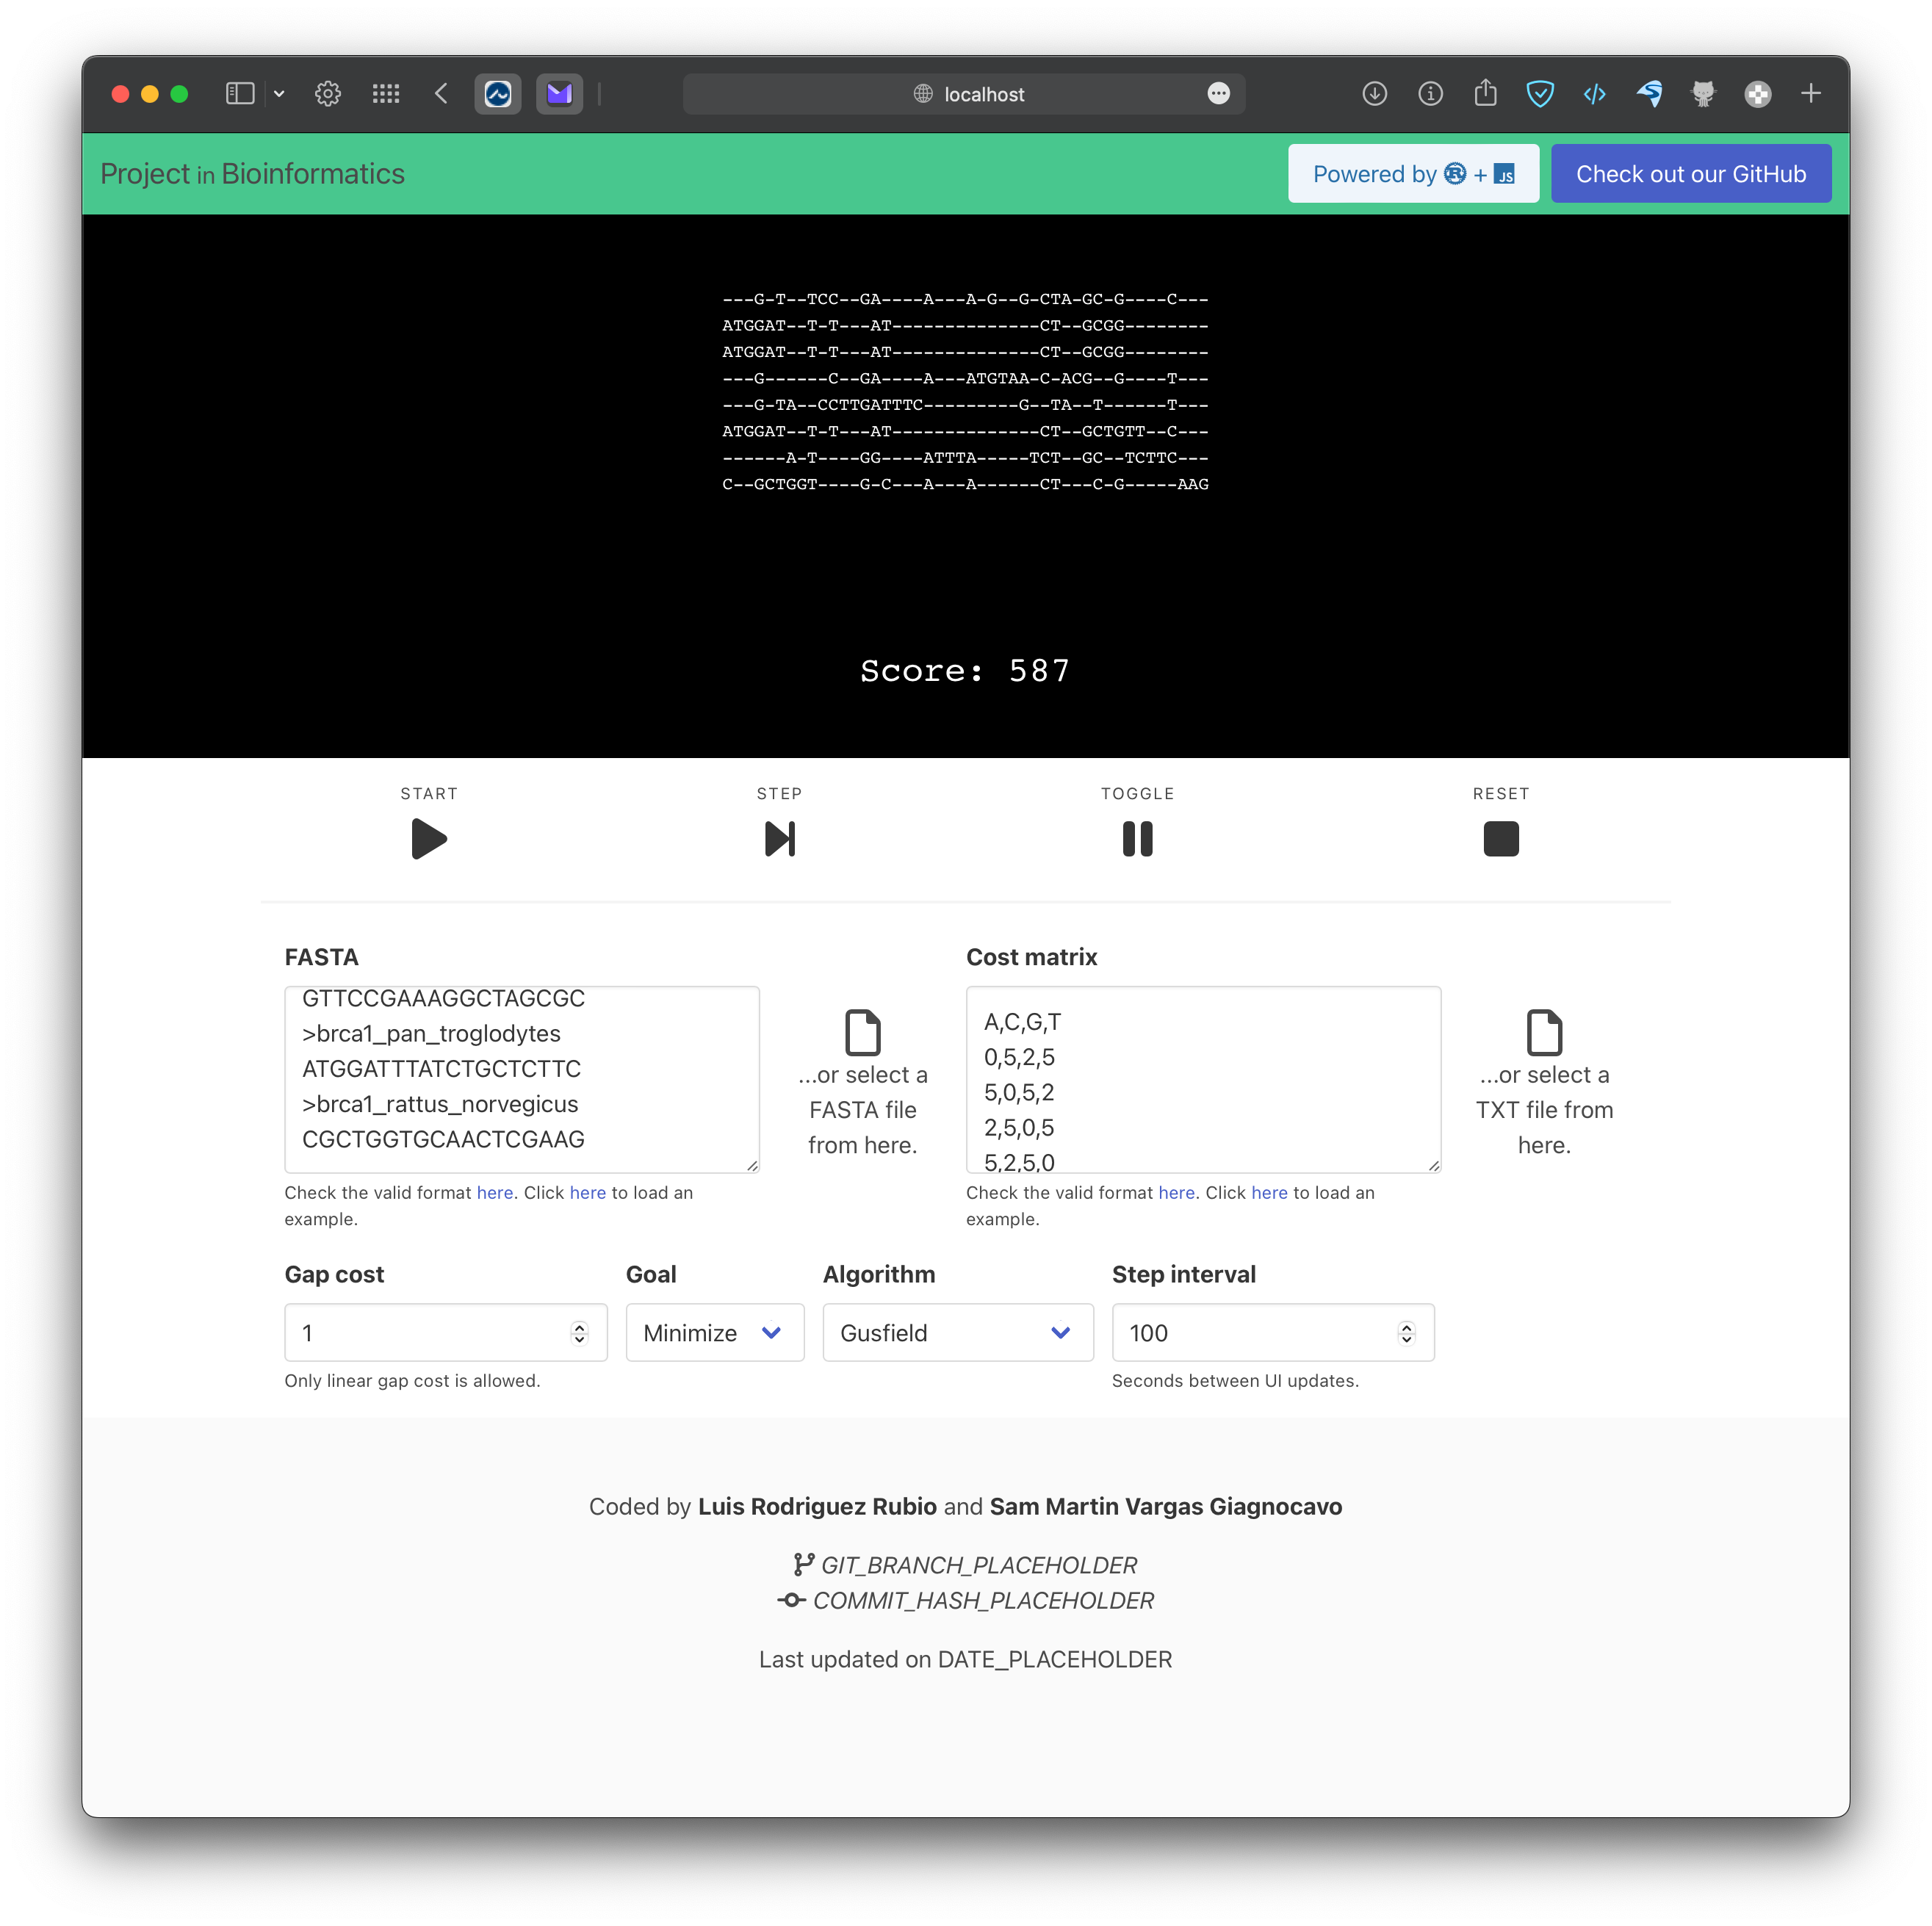
\includegraphics[width=0.8\textwidth]{report/webapp.png}
    \centering
    \caption{Overview of the final website.}
    \label{fig:webapp}
\end{figure}

\chapter{Evaluation \& Conclusion}
\label{cha:evaluation}

Evaluation and testing was thought of from the initial stages of development. \textit{cargo}, Rust's package manager, allows for benchmarking\footnote{https://doc.rust-lang.org/cargo/commands/cargo-bench.html} and unit testing\footnote{https://doc.rust-lang.org/cargo/commands/cargo-test.html} to be included with ease in any Rust project. In our project, two folders, \textit{benchmarks} and \textit{tests}, have been added to the \textit{src} folder.

To test the implementation, two ``types" of test data were used: Sequenced data and completely randomized data. Amongst the sequenced data two sets were tested, a collection of chromosomes from \href{https://www.ncbi.nlm.nih.gov/assembly/GCF_000001635.27/}{\textit{mus musculus'} reference genome} and sequences from different \href{https://viralzone.expasy.org/9556}{SARS-CoV-2 variants}. In addition to the completely randomized scenario, we wanted to test the algorithm's capability in two ``realistic" scenarios where we can expect considerably different rates of divergence between sequences.

For each iteration of our tests we decided to use a fairly simple score matrix. The reasoning for not using other popular score matrices such as BLOSUM or PAM is mostly due to our lack of experience with most of the well-established matrices and resources such as \cite{pearson2013selecting}, which argue that DNA sequence comparison is much less sensitive than protein sequence comparison.

As for variations regarding the algorithm, two additions have been added specifically for the testing phase. In one, instead of using the default merge-order vector from our Kruskal implementation we invert the steps, this time starting from the end. In the other variation, we randomize the merging steps. The goal is to further explore the effect of the merging phase has in our score.

Before going through the final results of our comparison, we briefly explain how to compile, set up and test our solution. The code is hosted at \url{https://github.com/Lewis-11/PiB}. Users can either clone the git repository locally or download a ZIP file containing the source code. Within the root of the project, \textit{cargo build -{}-release} - which has to be run from the command line prompt - will generate an executable binary inside the \textit{target/release} folder. As a requirement, users should have both, the Rust compiler and Cargo installed. An execution of the program looks as follows: \textit{./target/release/msa mst --submat mat.txt sequences.fa}. For more info regarding the different options that can be specified, run \textit{./target/release/msa help}.

In order to verify that all unit tests are working as expected, users can run \textit{cargo test} from the root of the project. The tool will output in the command line the status of each of the tests.

While performance was not a priority throughout development since we had to adapt our code for two different platforms, the \textit{cargo bench} command is available and will generate a detailed report comparing running times between the different algorithms. See \textit{section \ref{sec:criterion}} for more information.

Users that in addition want to deploy the web interface, need to install and run the \textit{wasm-pack build} command from the command prompt. Once the WASM files are generated, the user can go inside the \textit{www} folder and run \textit{npm start} to start a local instance of the website at \textit{localhost:8080}. However, in the repository's \textit{README.md} file there is already a link to an external website that hosts all of the active git branches\footnote{A personal server is used so there is no guarantee that the website will be operational at all times.}. Now that we have introduced the setup we proceed to talk more extensively about our results.

\section{Scoring comparison}

In accordance with the previously discussed methodology, we recorded the score of utilizing four distinct guide tree configurations. These configurations included a star-shaped tree generated via Gusfield's ``center string" algorithm, a minimum spanning tree (MST) constructed utilizing the Disjoint Set Union implementation of Kruskal's algorithm, and two variations of the aforementioned MST. The variations comprised of reversing the order of merges, beginning with the most dissimilar sequences within the MST, and the other variation involved randomly shuffling the order of the merges.

We have evaluated each of the four implementations with the three data sets mentioned in this chapter's introduction. The ``real-world" FASTAS range from sequences of relatively small length (100-600 characters) to larger sequences of 30,000 and 23,000 characters. With regards to the artificially generated sequences, we have examined groups of 5 and 10 sequences of lengths 1000, 5000, and 10,000.

We first compared the score ratio of our implementation of Kruskal's algorithm with Gusfield's score. A lower ratio indicates an improvement in Gusfield's score. We calculated the average score ratio for each test by combining the lengths of the sequences. As shown in \textit{Figure \ref{fig:gusVSkruskal}}, the results were mostly better, with an average ratio of 0.67, which translates to a 33\% improvement. It's important to keep in mind that this comparison is based on our observations and there's yet to be proof that MSTs lead to a higher alignment quality.

\begin{figure}[H]
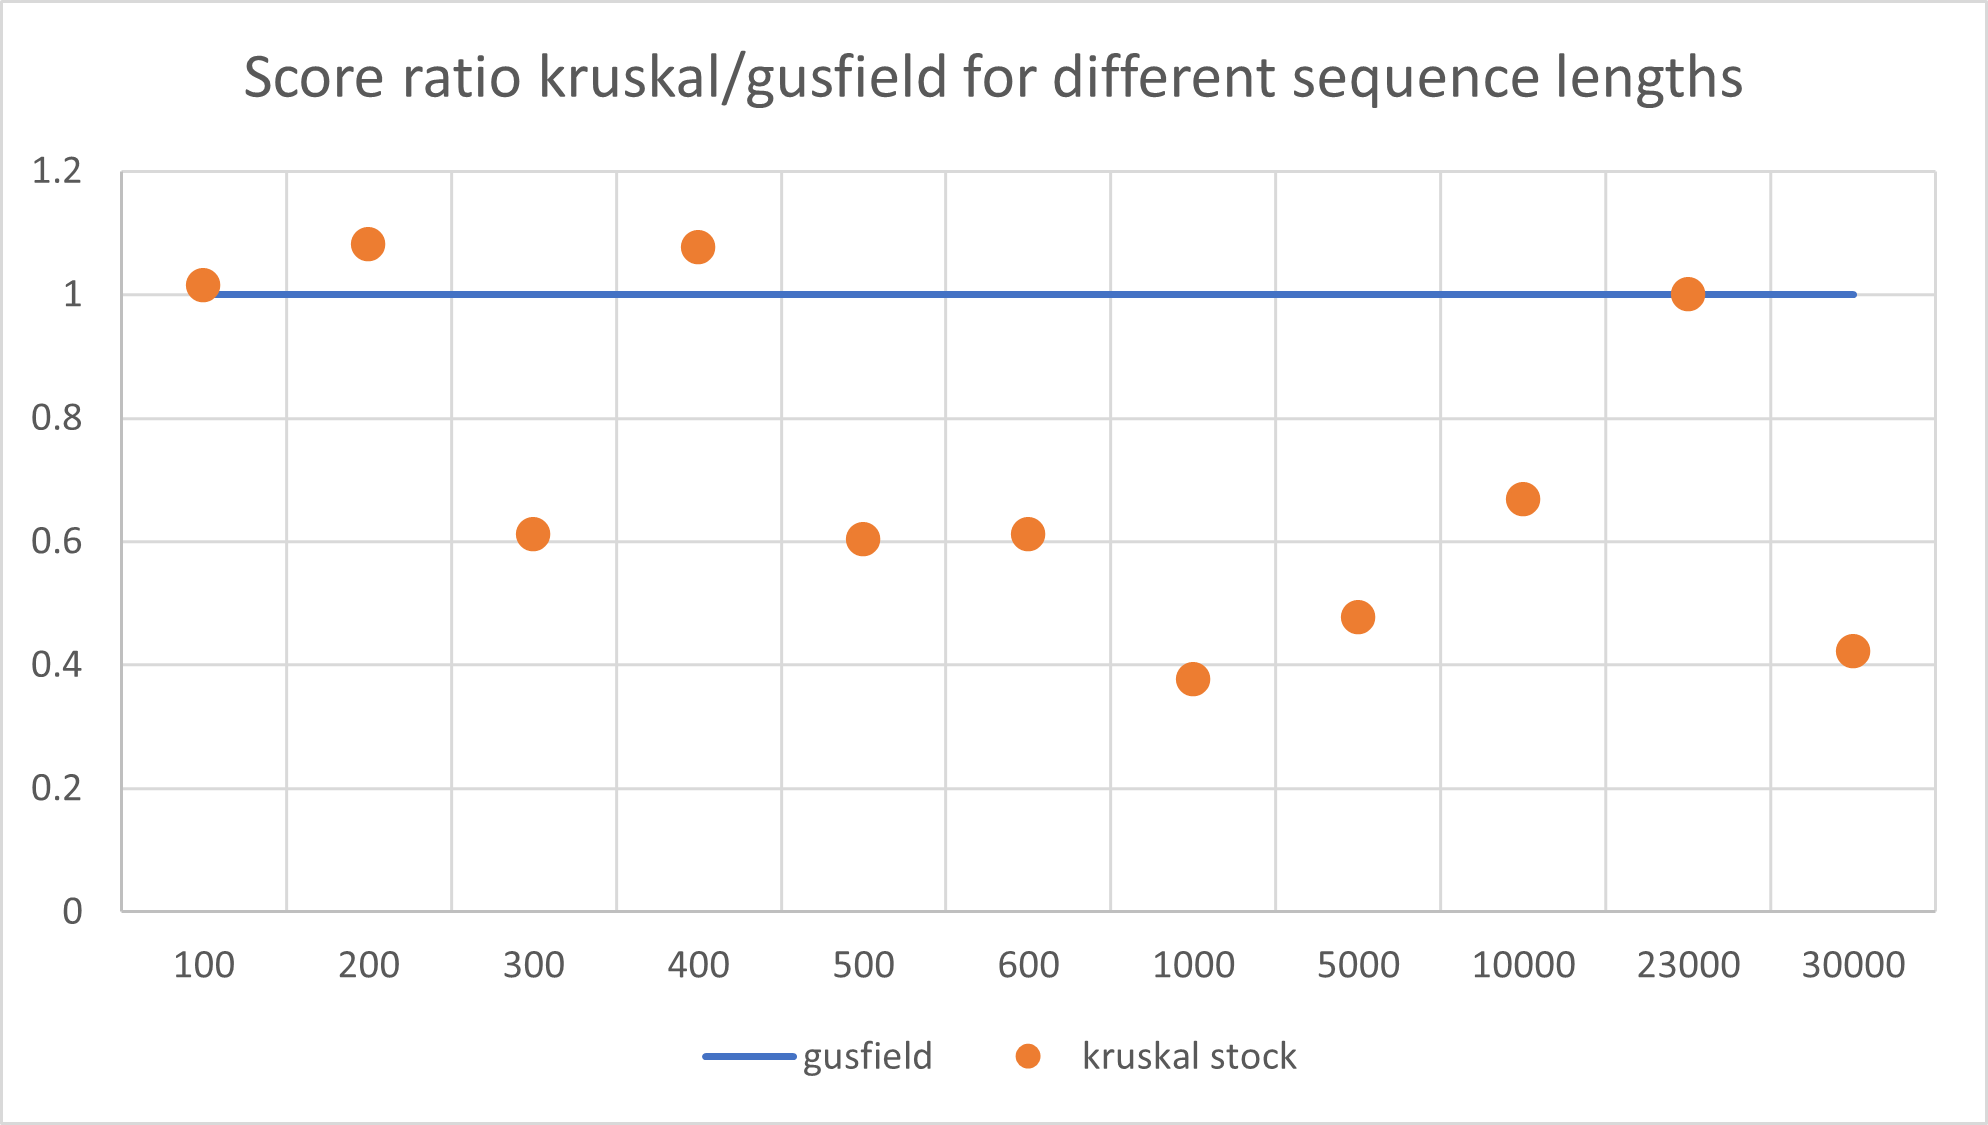
\includegraphics[width=0.8\textwidth]{report/kruskalVSgudfield.png}
\centering
\caption{Score ratio between Gusfield's "center string" \& Kruskal's MST as guide tree for different sequence lengths.}
\label{fig:gusVSkruskal}
\end{figure}

We also evaluated various MST alternatives that modify the order in which sequences are merged following the MST. The standard approach merges sequences with smaller scores (more similar sequences) first, while the reversed version starts with sequences with higher scores (more dissimilar sequences), and the last one is a random order. To determine if these alternatives show an improvement over the standard MST (lower scores first), we calculated a score ratio between the alternatives and the standard MST, as we did before. The results can be seen in \textit{Figure \ref{fig:kruskalVSkruskal}}. 

\begin{figure}[H]
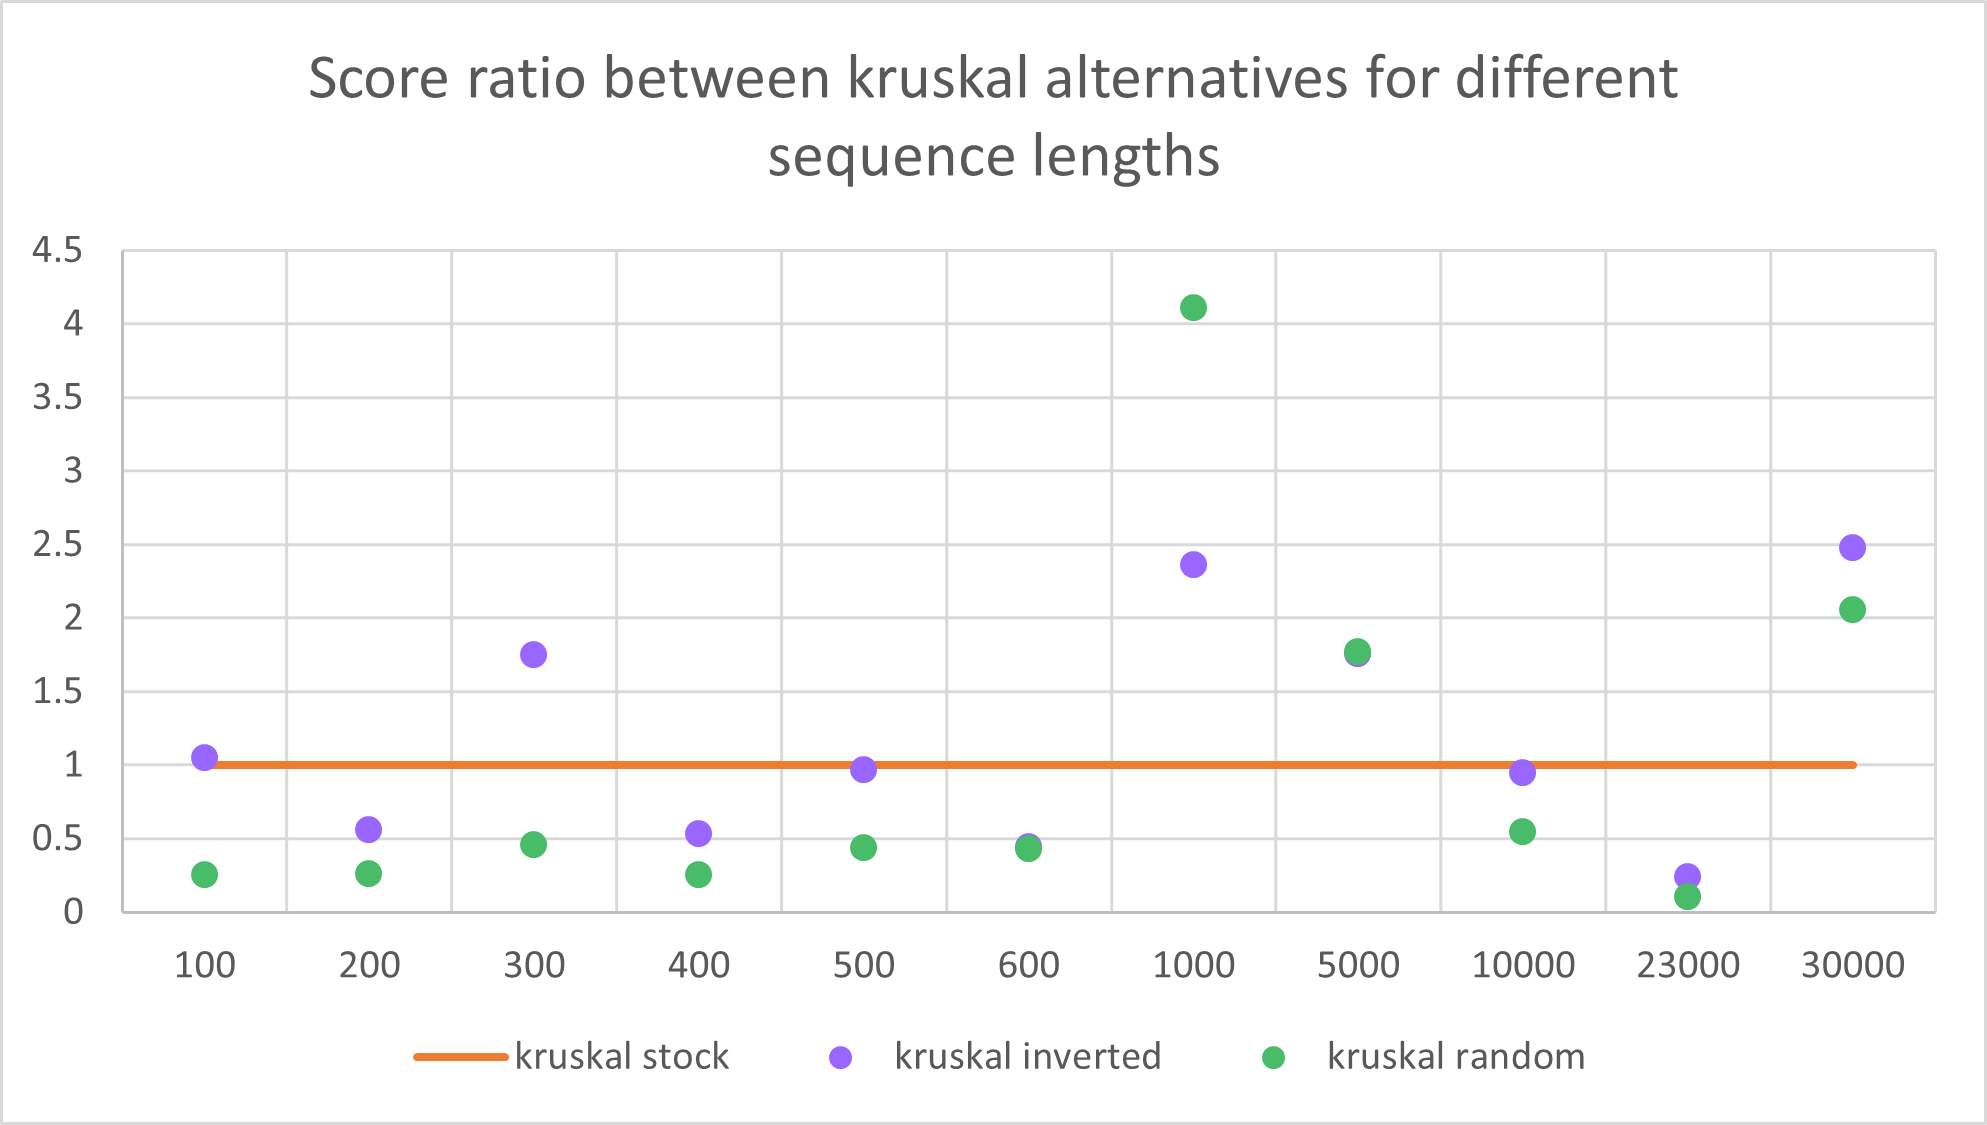
\includegraphics[width=0.8\textwidth]{report/kruskalsVSkruskal.png}
\centering
\caption{Score ratio between Kruskal's MST alternatives for different sequence lengths.}
\label{fig:kruskalVSkruskal}
\end{figure}

The average ratio for the inverted order is 1.25 and for the random order is 1.06, which represents a 25\% and 6\% decrease in performance (since we aim for a low ratio to minimize scores). Thus, based on our observations, the standard MST order is the one that yields the best results on average.

Based on our observations, it is notable that the differences between using Gusfield's star-tree and Kruskal's MST become more apparent when the number of sequences (k) is larger. This can be observed by comparing \textit{Figure \ref{fig:chart-2}}, which shows results for 5 sequences, with \textit{Figure \ref{fig:chart-3}}, which shows results for different sequence lengths. This trend can also be observed in real-world data, such as the comparison of different mouse sequences in \textit{Figure \ref{fig:chart-5}}, which have 5 sequences, versus the results obtained from aligning 9 sequences of COVID variants in \textit{Figure \ref{fig:chart-4}}, where we can see a more significant improvement from Kruskal's alternative when compared to Gusfield's method.

\begin{figure}[H]
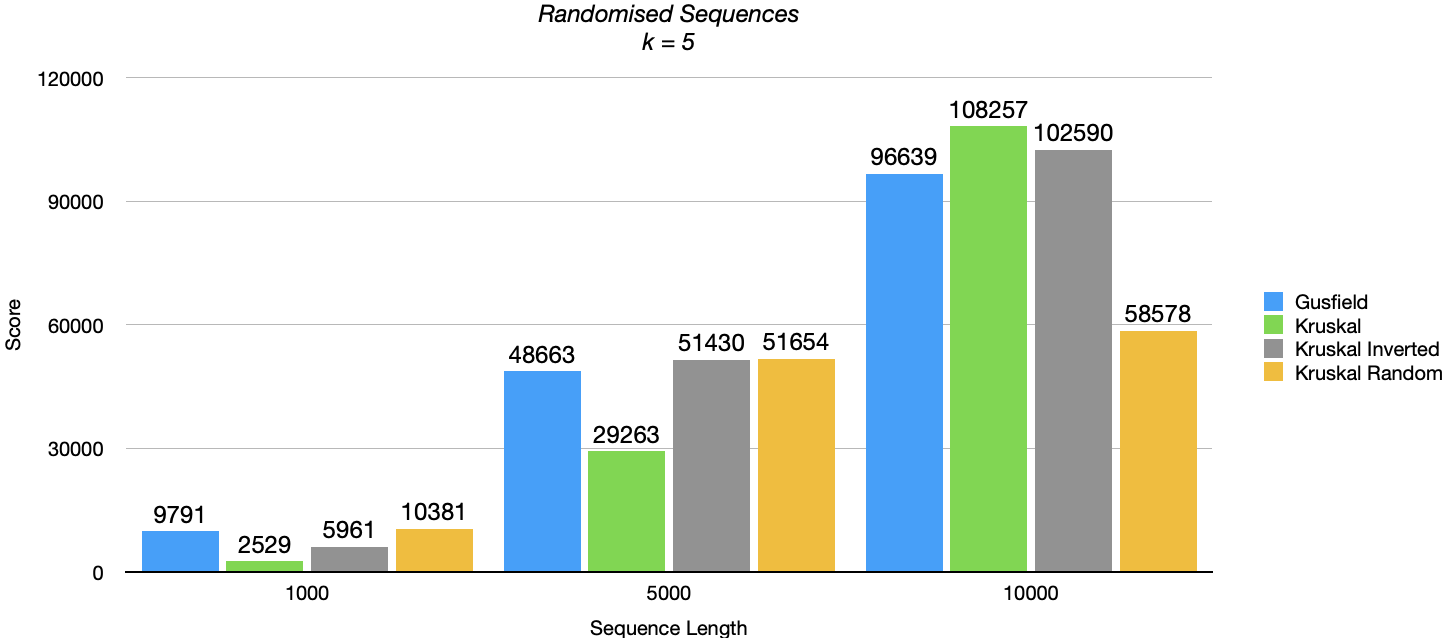
\includegraphics[width=0.8\textwidth]{report/chart-2.png}
\centering
\caption{Scores from aligning 5 randomized sequences of multiple sizes.}
\label{fig:chart-2}
\end{figure}

\begin{figure}[H]
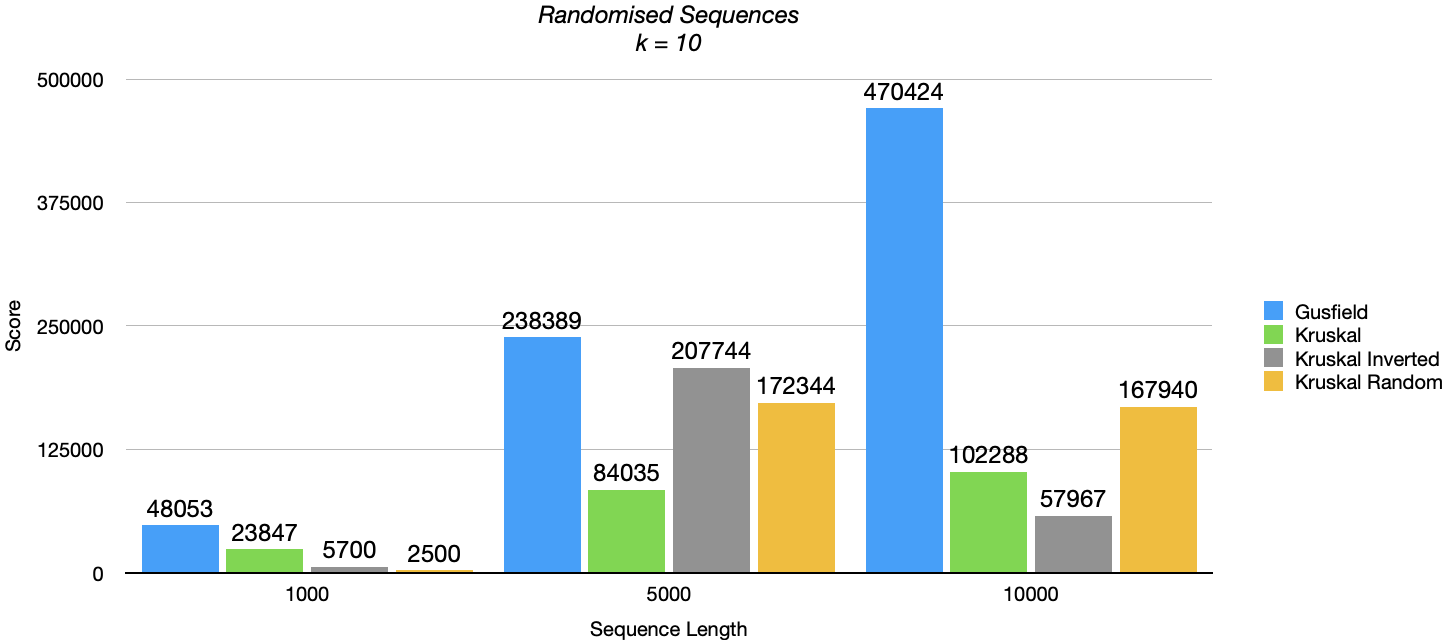
\includegraphics[width=0.8\textwidth]{report/chart-3.png}
\centering
\caption{Scores from aligning 10 randomized sequences of multiple sizes.}
\label{fig:chart-3}
\end{figure}

\begin{figure}[H]
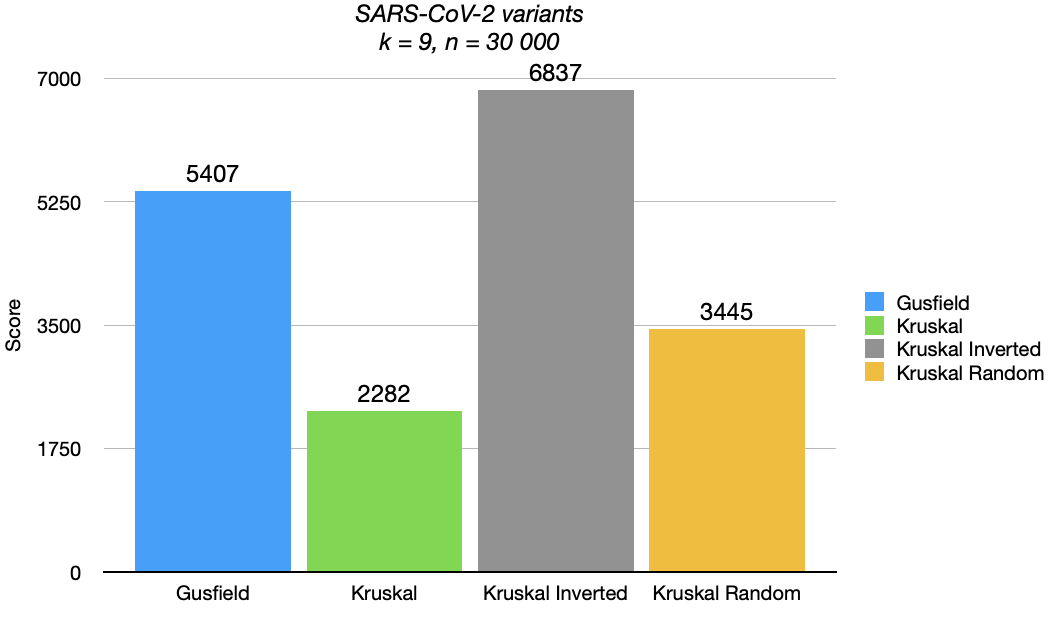
\includegraphics[width=0.8\textwidth]{report/chart-4.png}
\centering
\caption{Scores from aligning 9 SARS-CoV-2 variants.}
\label{fig:chart-4}
\end{figure}

\begin{figure}[H]
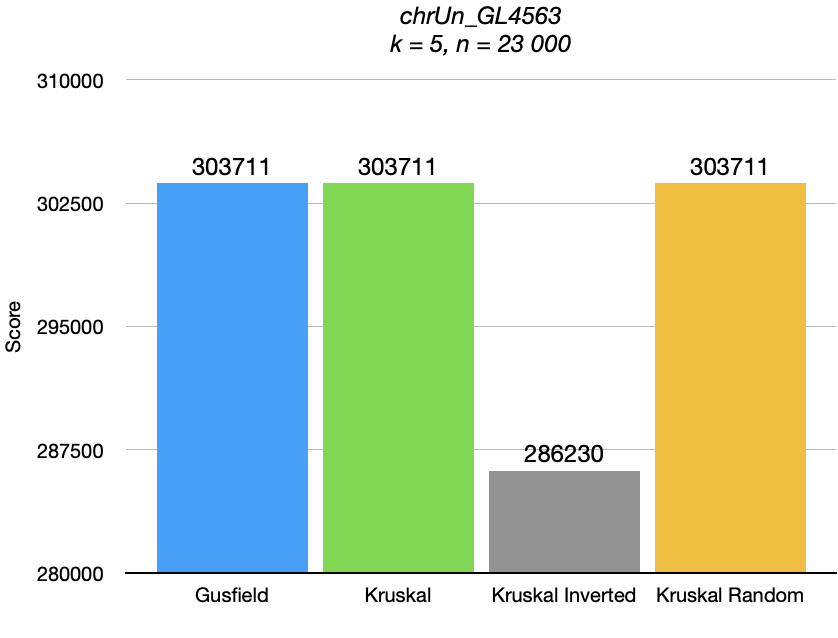
\includegraphics[width=0.8\textwidth]{report/chart-5.png}
\centering
\caption{Scores from aligning 5 sequences from the \textit{mus musculus} reference genome.}
\label{fig:chart-5}
\end{figure}

This can be attributed to the fact that an increase in the number of sequences leads to an increase in the number of nodes in the adjacency matrix of alignments. This also means that there are more potential trees. This has been demonstrated in \textit{Figure \ref{fig:chart-5}}, with the mouse dataset, Gusfield, standard Kruskal, and random Kruskal all obtained the same score. This was due to the fact that the guide tree was similar in every case. In cases where there are very few sequences, random order of kruskals MST yields the best results as can be seen in \textit{Figure \ref{fig:chart-1}}.


\begin{figure}[H]
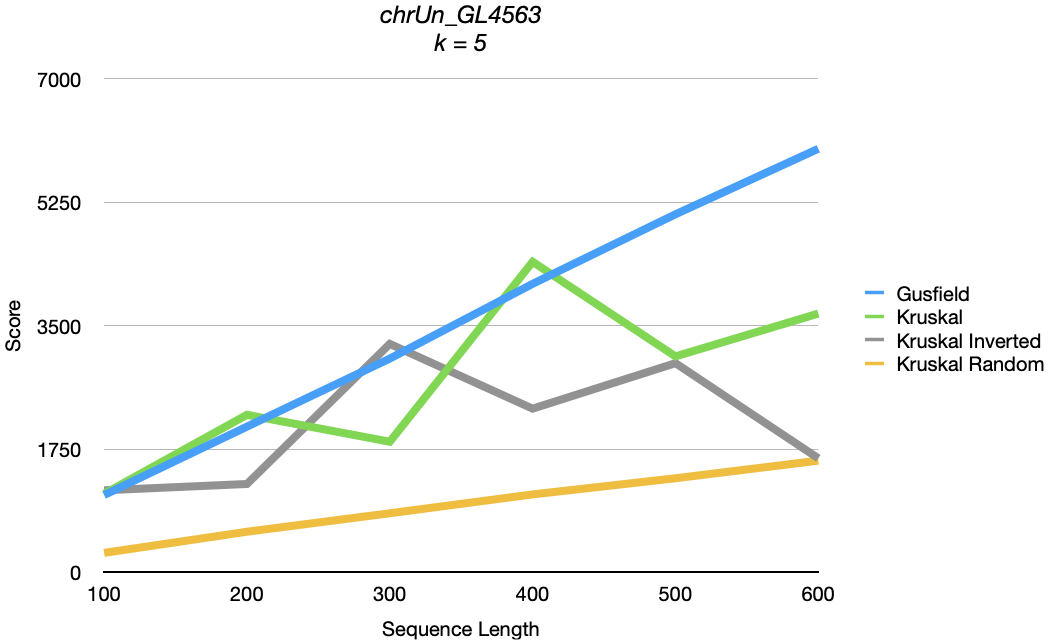
\includegraphics[width=0.8\textwidth]{report/chart-1.png}
\centering
\caption{Scores from aligning 5 differently-sized sequences from the \textit{mus musculus} reference genome.}
\label{fig:chart-1}
\end{figure}

As a final note, in \textit{chapter \ref{cha:arch--impl}} we mentioned the increased running time of adding Kruskal's algorithm on top of Gusfield's. \textit{Figure \ref{fig:running-times}} clearly shows that in theory there is some overhead most of the processing is done aligning both sequences and clusters. The base Gusfield implementation and Gusfield + Kruskal implementation offer near identical running times.

\begin{figure}[h]
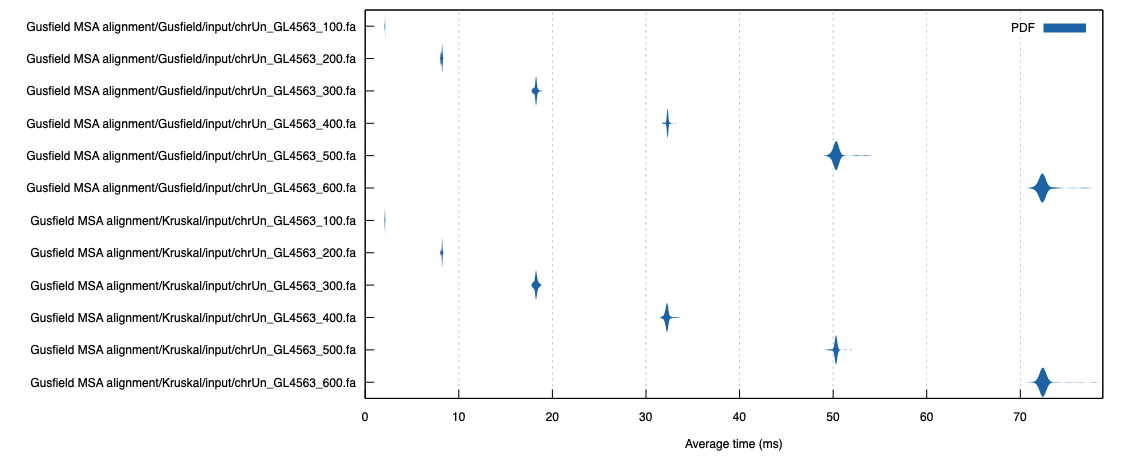
\includegraphics[width=0.8\textwidth]{report/runing-times.png}
\centering
\caption{Running times from a series of tests comparing the base Gusfield implementation with the improved one.}
\label{fig:running-times}
\end{figure}

\section{Conclusion and Future Work}
As described in the introduction, we were interested in the possibilities this project had to offer both from a bio-informatics and computer science standpoint. While the diverging results don't offer the clear conclusion we were hoping for, we still found the evaluation phase interesting as it showed how small changes can greatly change the end result. Further testing could shed some light on the effects not only the different variations of the Kruskal have but also what type of algorithm should be used depending on the type of sequences we are working with (e.g. extremely similar sequences might achieve a better alignment with a certain algorithm).

Regarding possible improvements if the project were to be continued, optimization and visualization could be the next major areas to upgrade. In multiple instances our Rust implementation stores redundant data, hence reducing the memory footprint would be ideal. Visualization-wise, the initial prototypes that were ideated in the early stages proved too ambitious for the scope of the project but would make the website that was developed for the project significantly more functional. 

Another limitation, which is also present in the visualization but cascaded from our Rust implementation, is the lack of sequence identifiers in the resulting cluster.

Despite the limitations, we consider the project a great learning experience since we expanded our knowledge in areas that we didn't have an opportunity to expand on during courses like \textit{Algorithms in Bioinformatics} and \textit{Genome Scale Algorithms} (e.g. trying to optimize Gusfield's 2-approximation algorithm and the alignment of clusters as opposed to single sequences). In addition, from a more practical point of view, we learned to work with two relatively new tools such as Rust and WebAssembly. Both of which, we consider, will be useful in future projects.

\appendix
\cleardoublepage

\chapter{Appendix}
\label{cha:an-appendix}

\section{Our GitHub's CD/CI configuration}
\label{sec:github-ci}
In order to quickly and automatically build, test and deploy our code we defined two \textit{GitHub Action} jobs. Part of one can be seen in the code listing below. Here we can see how we install \textit{wasm-pack}, build and convert our Rust code into WebAssembly and do some minor modifications to the website before sending the compiled version to a web server.

\lstset{basicstyle=\ttfamily\scriptsize}
\begin{lstlisting}[language=YAML,numbers=none]
...

jobs:
  build:
    runs-on: ubuntu-latest
    steps:
    - uses: actions/checkout@v3
    - name: Install wasm-pack
      run: curl https://rustwasm.github.io/wasm-pack/installer/init.sh -sSf | sh
    - name: Generate pkg files
      run: wasm-pack build
    - name: Replace GIT_BRANCH_PLACEHOLDER, COMMIT_HASH_PLACEHOLDER and DATE_PLACEHOLDER
      run: |
        cd www
        sed -i 's/GIT_BRANCH_PLACEHOLDER/'"${GITHUB_REF##*/}"'/g' index.html
        sed -i 's/COMMIT_HASH_PLACEHOLDER/'"${GITHUB_SHA}"'/g' index.html
        sed -i 's/DATE_PLACEHOLDER/'"$(TZ=Europe/Copenhagen date)"'/g' index.html
    - name: Compile Webpack
      run: cd www && npm install && npm run build
    - name: Copy to server
      uses: easingthemes/ssh-deploy@main
      env:
        SSH_PRIVATE_KEY: ${{ secrets.RSA_KEY }}
        REMOTE_HOST: ${{ secrets.HOST }}
        SOURCE: "msa/www/dist/"
        REMOTE_USER: ${{ secrets.REMOTE_USER }}
        REMOTE_PORT: ${{ secrets.PORT }}
        TARGET: "builds/${GITHUB_REF##*/}"
\end{lstlisting}

The web server is set up in a way that allows the viewing of different branches. The idea behind this setup was to make testing as easy as possible. \textit{Figure \ref{fig:ci-branch-index}} shows the index page of the server.

\begin{figure}[h]
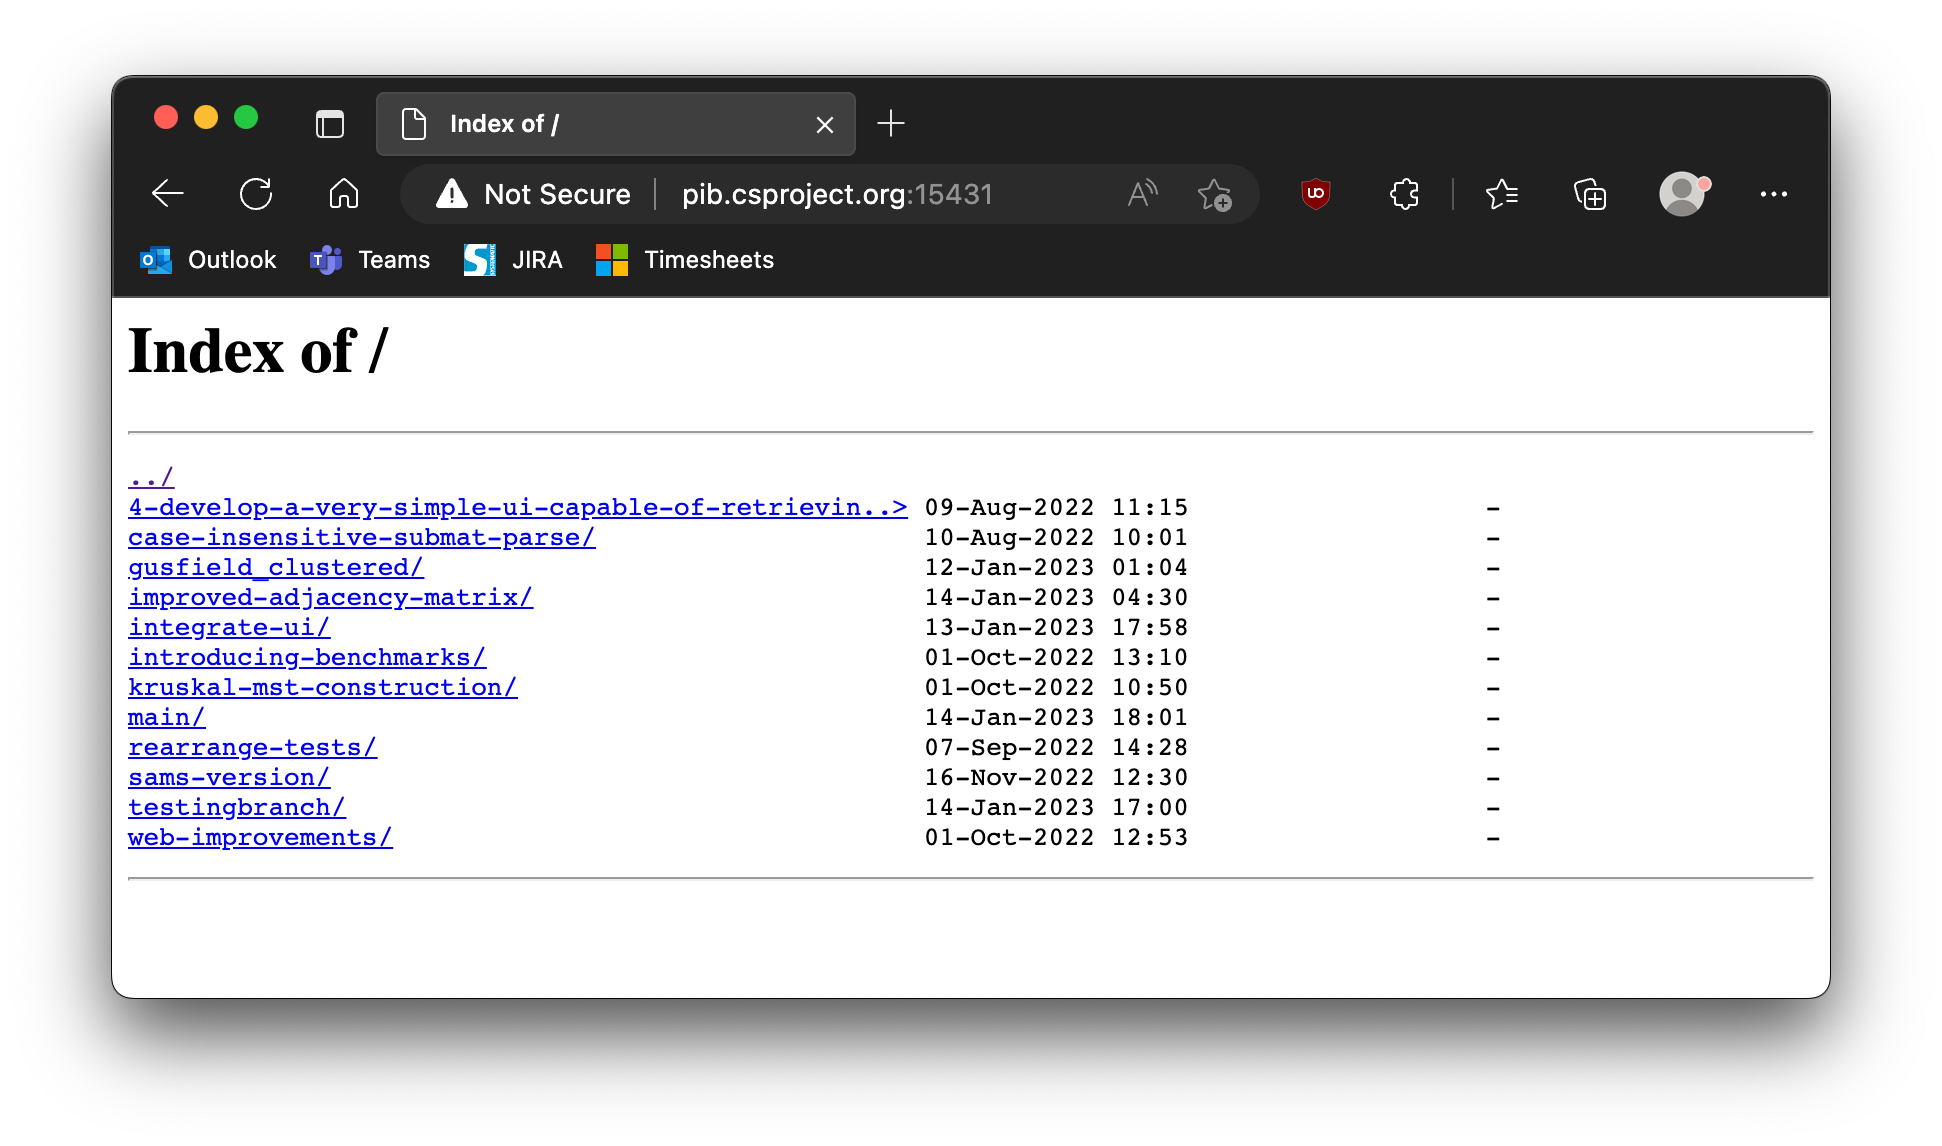
\includegraphics[width=0.8\textwidth]{report/ci-branch-index.png}
\centering
\caption{Root of the custom server used for the development of the solution.}
\label{fig:ci-branch-index}
\end{figure}

\FloatBarrier

\section{Running times generated by the \textit{criterion} library}
\label{sec:criterion}
Running the \textit{cargo bench} command will run all of the benchmarks defined within the \textit{Cargo.toml} file. The \textit{criterion} library has been used in order to automate most of the prior (e.g. a test warm up) and subsequent (e.g. computing the standard deviation) steps of the benchmarking process. An example of the generated HTML file can be seen in \textit{Figure \ref{fig:criterion}}. Locally, this file is located inside the \textit{./target/criterion/Gusfield MSA alignment/report} folder.

\begin{figure}[h]
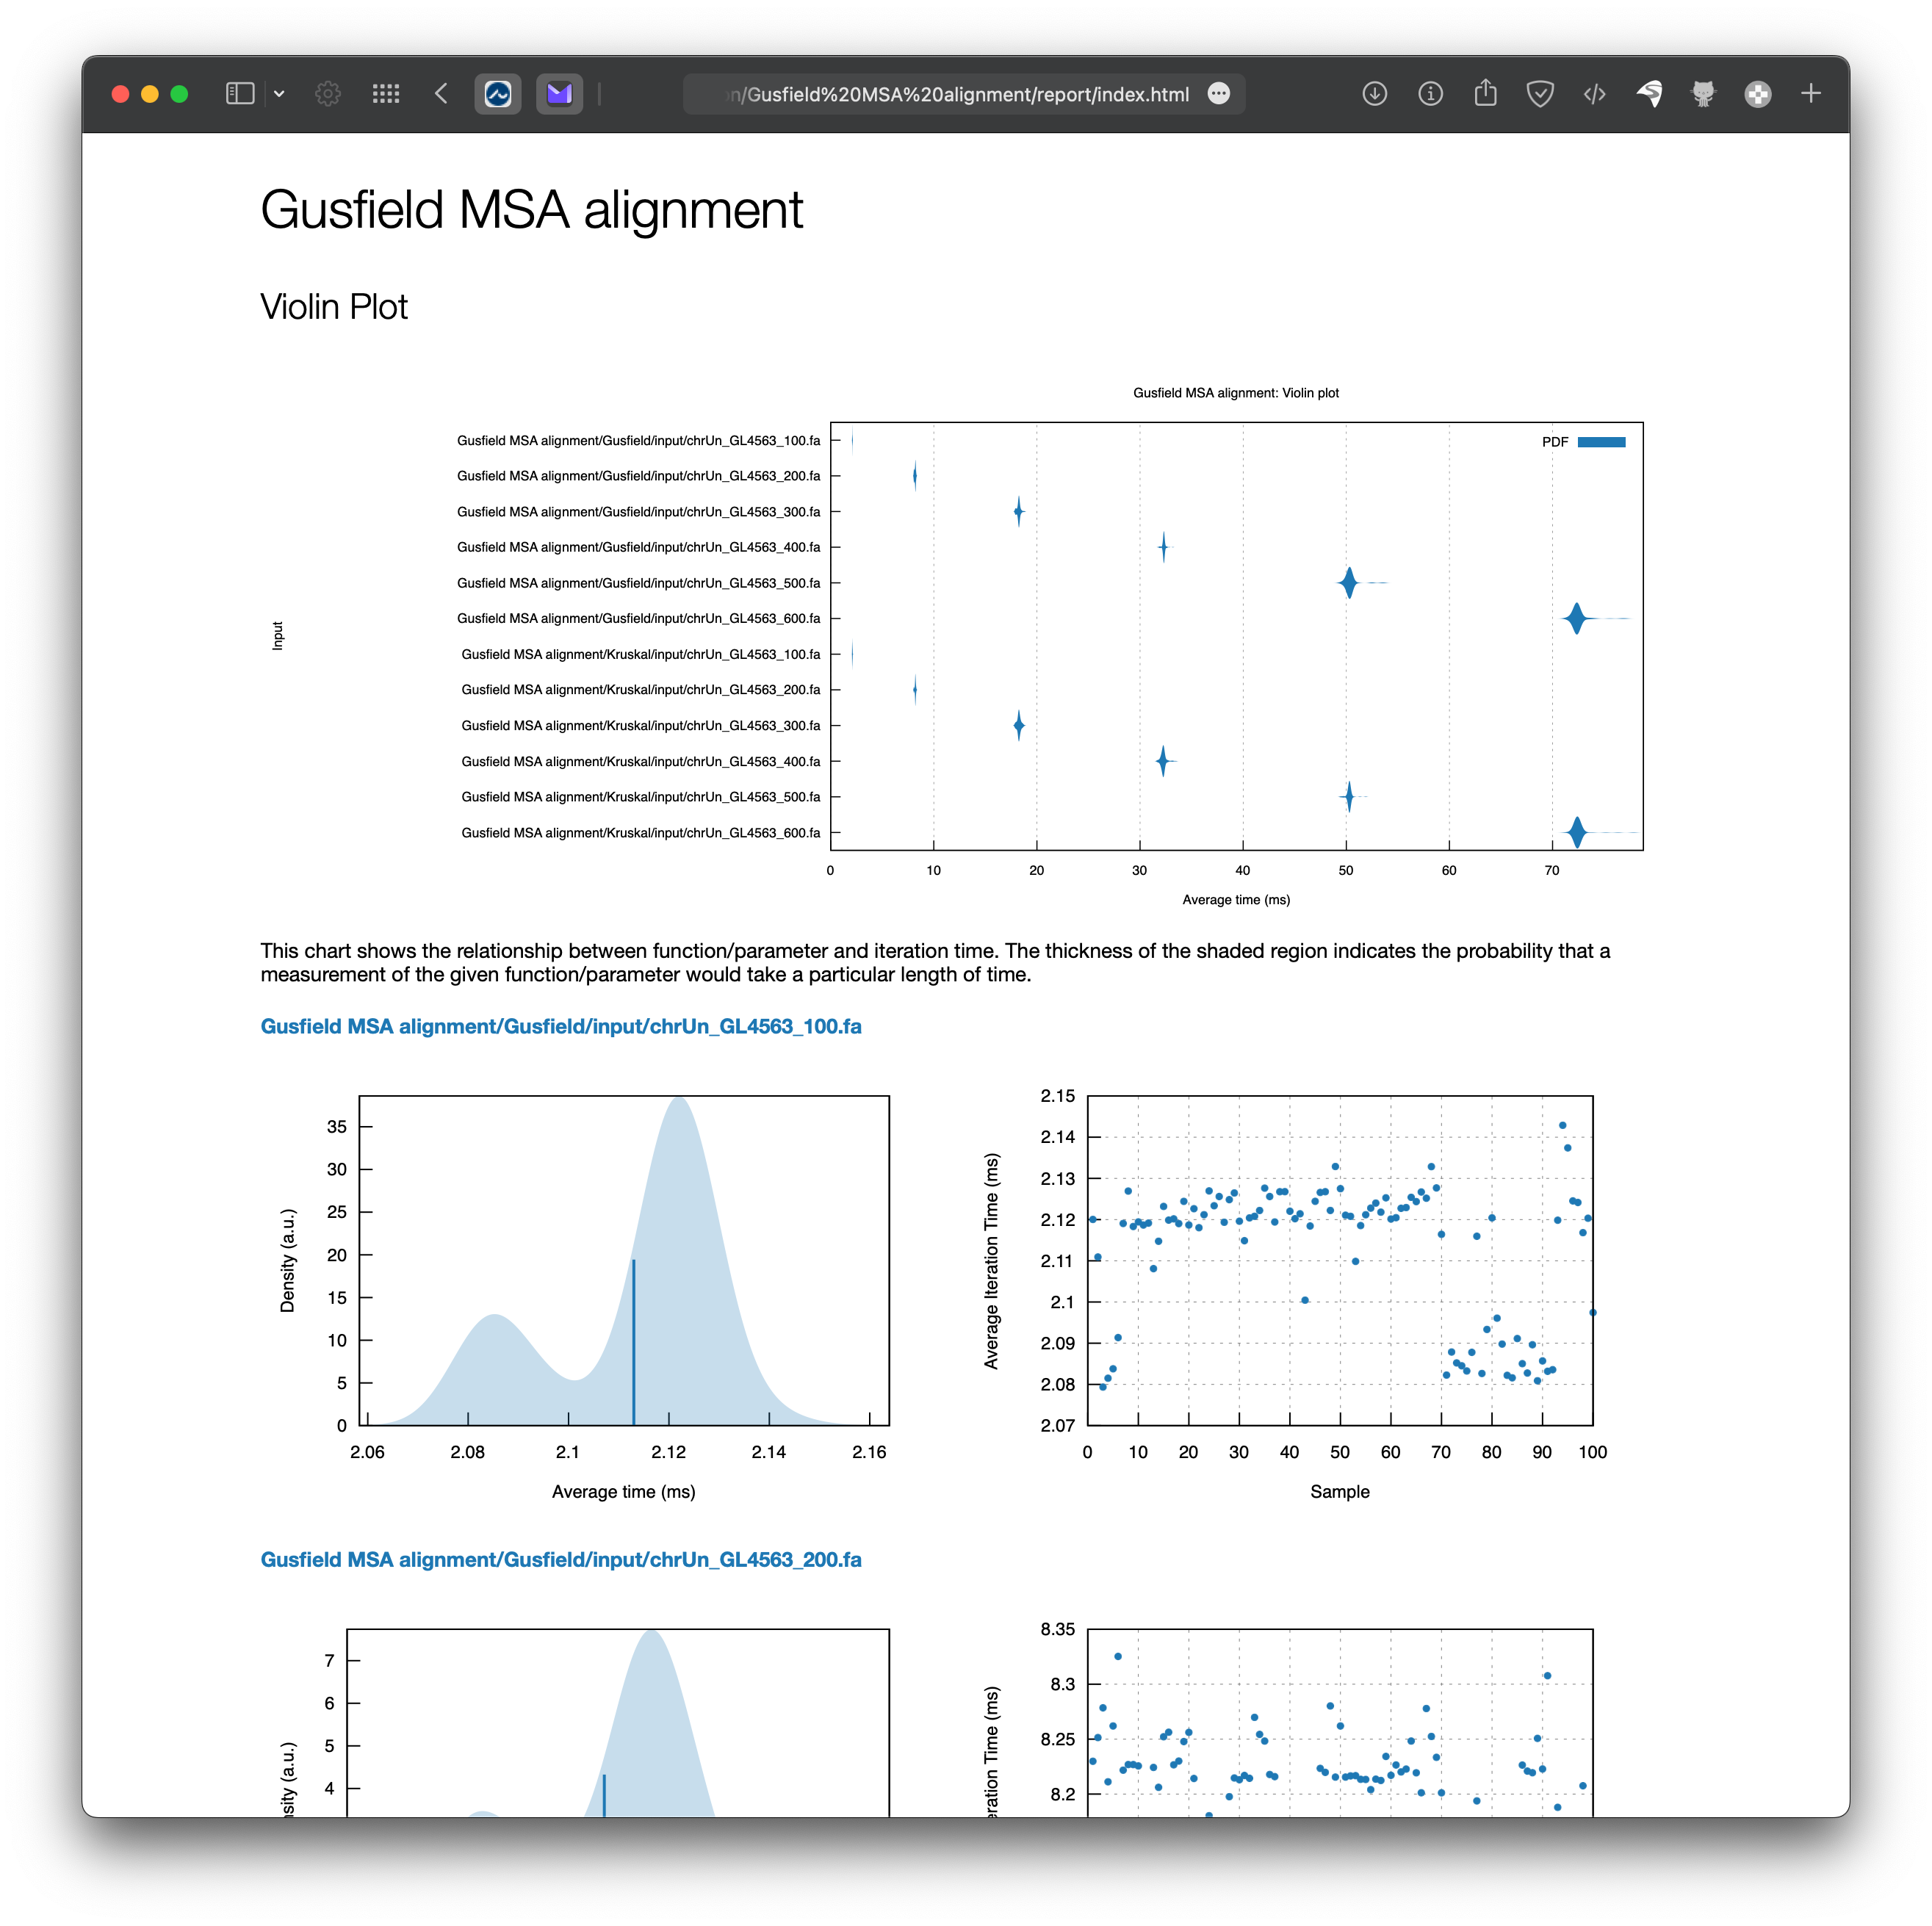
\includegraphics[width=0.8\textwidth]{report/criterion.png}
\centering
\caption{Generated output from \textit{criterion}.}
\label{fig:criterion}
\end{figure}


%********************************************************************
% Other Stuff in the Back
%*******************************************************
\cleardoublepage%********************************************************************
% Bibliography
%*******************************************************
% work-around to have small caps also here in the headline
\manualmark
\markboth{\spacedlowsmallcaps{\bibname}}{\spacedlowsmallcaps{\bibname}} % work-around to have small caps also
%\phantomsection 
\refstepcounter{dummy}
\addtocontents{toc}{\protect\vspace{\beforebibskip}} % to have the bib a bit from the rest in the toc
\addcontentsline{toc}{chapter}{\tocEntry{\bibname}}
\label{app:bibliography}
\printbibliography


% ********************************************************************
% Game Over: Restore, Restart, or Quit?
%*******************************************************
\end{document}
% ********************************************************************

%%% Local Variables:
%%% mode: latex
%%% TeX-master: t
%%% End:
